% Options for packages loaded elsewhere
\PassOptionsToPackage{unicode}{hyperref}
\PassOptionsToPackage{hyphens}{url}
\PassOptionsToPackage{dvipsnames,svgnames,x11names}{xcolor}
%
\documentclass[
  letterpaper,
  DIV=11,
  numbers=noendperiod]{scrartcl}

\usepackage{amsmath,amssymb}
\usepackage{lmodern}
\usepackage{iftex}
\ifPDFTeX
  \usepackage[T1]{fontenc}
  \usepackage[utf8]{inputenc}
  \usepackage{textcomp} % provide euro and other symbols
\else % if luatex or xetex
  \usepackage{unicode-math}
  \defaultfontfeatures{Scale=MatchLowercase}
  \defaultfontfeatures[\rmfamily]{Ligatures=TeX,Scale=1}
\fi
% Use upquote if available, for straight quotes in verbatim environments
\IfFileExists{upquote.sty}{\usepackage{upquote}}{}
\IfFileExists{microtype.sty}{% use microtype if available
  \usepackage[]{microtype}
  \UseMicrotypeSet[protrusion]{basicmath} % disable protrusion for tt fonts
}{}
\makeatletter
\@ifundefined{KOMAClassName}{% if non-KOMA class
  \IfFileExists{parskip.sty}{%
    \usepackage{parskip}
  }{% else
    \setlength{\parindent}{0pt}
    \setlength{\parskip}{6pt plus 2pt minus 1pt}}
}{% if KOMA class
  \KOMAoptions{parskip=half}}
\makeatother
\usepackage{xcolor}
\setlength{\emergencystretch}{3em} % prevent overfull lines
\setcounter{secnumdepth}{5}
% Make \paragraph and \subparagraph free-standing
\ifx\paragraph\undefined\else
  \let\oldparagraph\paragraph
  \renewcommand{\paragraph}[1]{\oldparagraph{#1}\mbox{}}
\fi
\ifx\subparagraph\undefined\else
  \let\oldsubparagraph\subparagraph
  \renewcommand{\subparagraph}[1]{\oldsubparagraph{#1}\mbox{}}
\fi


\providecommand{\tightlist}{%
  \setlength{\itemsep}{0pt}\setlength{\parskip}{0pt}}\usepackage{longtable,booktabs,array}
\usepackage{calc} % for calculating minipage widths
% Correct order of tables after \paragraph or \subparagraph
\usepackage{etoolbox}
\makeatletter
\patchcmd\longtable{\par}{\if@noskipsec\mbox{}\fi\par}{}{}
\makeatother
% Allow footnotes in longtable head/foot
\IfFileExists{footnotehyper.sty}{\usepackage{footnotehyper}}{\usepackage{footnote}}
\makesavenoteenv{longtable}
\usepackage{graphicx}
\makeatletter
\def\maxwidth{\ifdim\Gin@nat@width>\linewidth\linewidth\else\Gin@nat@width\fi}
\def\maxheight{\ifdim\Gin@nat@height>\textheight\textheight\else\Gin@nat@height\fi}
\makeatother
% Scale images if necessary, so that they will not overflow the page
% margins by default, and it is still possible to overwrite the defaults
% using explicit options in \includegraphics[width, height, ...]{}
\setkeys{Gin}{width=\maxwidth,height=\maxheight,keepaspectratio}
% Set default figure placement to htbp
\makeatletter
\def\fps@figure{htbp}
\makeatother

\KOMAoption{captions}{tableheading}
\makeatletter
\makeatother
\makeatletter
\makeatother
\makeatletter
\@ifpackageloaded{caption}{}{\usepackage{caption}}
\AtBeginDocument{%
\ifdefined\contentsname
  \renewcommand*\contentsname{Table of contents}
\else
  \newcommand\contentsname{Table of contents}
\fi
\ifdefined\listfigurename
  \renewcommand*\listfigurename{List of Figures}
\else
  \newcommand\listfigurename{List of Figures}
\fi
\ifdefined\listtablename
  \renewcommand*\listtablename{List of Tables}
\else
  \newcommand\listtablename{List of Tables}
\fi
\ifdefined\figurename
  \renewcommand*\figurename{Figure}
\else
  \newcommand\figurename{Figure}
\fi
\ifdefined\tablename
  \renewcommand*\tablename{Table}
\else
  \newcommand\tablename{Table}
\fi
}
\@ifpackageloaded{float}{}{\usepackage{float}}
\floatstyle{ruled}
\@ifundefined{c@chapter}{\newfloat{codelisting}{h}{lop}}{\newfloat{codelisting}{h}{lop}[chapter]}
\floatname{codelisting}{Listing}
\newcommand*\listoflistings{\listof{codelisting}{List of Listings}}
\makeatother
\makeatletter
\@ifpackageloaded{caption}{}{\usepackage{caption}}
\@ifpackageloaded{subcaption}{}{\usepackage{subcaption}}
\makeatother
\makeatletter
\@ifpackageloaded{tcolorbox}{}{\usepackage[many]{tcolorbox}}
\makeatother
\makeatletter
\@ifundefined{shadecolor}{\definecolor{shadecolor}{rgb}{.97, .97, .97}}
\makeatother
\makeatletter
\makeatother
\ifLuaTeX
  \usepackage{selnolig}  % disable illegal ligatures
\fi
\IfFileExists{bookmark.sty}{\usepackage{bookmark}}{\usepackage{hyperref}}
\IfFileExists{xurl.sty}{\usepackage{xurl}}{} % add URL line breaks if available
\urlstyle{same} % disable monospaced font for URLs
\hypersetup{
  pdftitle={Product Spaces},
  pdfauthor={Michael Betancourt},
  colorlinks=true,
  linkcolor={blue},
  filecolor={Maroon},
  citecolor={Blue},
  urlcolor={Blue},
  pdfcreator={LaTeX via pandoc}}

\title{Product Spaces}
\author{Michael Betancourt}
\date{April 2023}

\begin{document}
\maketitle
\ifdefined\Shaded\renewenvironment{Shaded}{\begin{tcolorbox}[frame hidden, sharp corners, interior hidden, boxrule=0pt, enhanced, borderline west={3pt}{0pt}{shadecolor}, breakable]}{\end{tcolorbox}}\fi

\renewcommand*\contentsname{Table of contents}
{
\hypersetup{linkcolor=}
\setcounter{tocdepth}{3}
\tableofcontents
}
Sometimes a system of applied interest can be adequately modeled with a
single
\href{https://betanalpha.github.io/assets/chapters_html/spaces.html}{space}.
When a system is too complicated for a single space we may be able to
model it with \emph{multiple spaces} at the same time. \emph{Product
spaces} integrate multiple component spaces together by first combining
both their underlying sets and their associated structures.

\hypertarget{product-sets}{%
\section{Product Sets}\label{product-sets}}

Product sets combine elements from multiple sets into \emph{composite}
elements. To develop this concept as cleanly as possible we'll first
investigate how to combine elements from finite sets before considering
the general case. Finally we'll investigate the behavior of subsets of
these product sets.

\hypertarget{finite-product-sets}{%
\subsection{Finite Product Sets}\label{finite-product-sets}}

Consider two finite sets, one with three elements, \[
X_{1} = \{ \Box, \clubsuit, \diamondsuit \},
\] and one with two elements, \[
X_{2} = \{ \heartsuit, \spadesuit \}.
\]

One way to combine these two sets together is to collect their
individual elements together into larger set, \[
X_{1} \cup X_{2} = \{ \Box, \clubsuit, \diamondsuit, \heartsuit, \spadesuit \}.
\] This concatenated set allows us to choose from any of the elements in
\(X_{1}\) and \(X_{2}\), but we can only choose \emph{only one element
at a time}.

In order to choose elements from \emph{both sets at the same time} we
need to account for all of the possible pairs of elements from \(X_{1}\)
and \(X_{2}\). This requires \emph{replicating} one of the sets for each
element in the other set.

For example we can replicate \(X_{2}\) three times, one for each element
of \(X_{1}\), to give the three distinct sets \begin{align*}
\{ \Box \} \times X_{2} &= \{ \heartsuit, \spadesuit \}
\\
\{ \clubsuit \} \times X_{2} &= \{ \heartsuit, \spadesuit \}
\\
\{ \diamondsuit \} \times X_{2} &= \{ \heartsuit, \spadesuit \}.
\end{align*} To differentiate between the elements of these replications
we can tag them with the corresponding element of \(X_{1}\), such as
\begin{align*}
\{ \Box \} \times X_{2}
&= \{ \heartsuit_{\Box}, \spadesuit_{\Box} \}
\\
\{ \clubsuit \} \times X_{2}
&= \{ \heartsuit_{\clubsuit}, \spadesuit_{\clubsuit} \}
\\
\{ \diamondsuit \} \times X_{2}
&= \{ \heartsuit_{\diamondsuit}, \spadesuit_{\diamondsuit} \}.
\end{align*} or \begin{align*}
\{ \Box \} \times X_{2}
&= \{ (\Box, \heartsuit), (\Box, \spadesuit) \}
\\
\{ \clubsuit \} \times X_{2}
&= \{ (\clubsuit, \heartsuit), (\clubsuit, \spadesuit) \}
\\
\{ \diamondsuit \} \times X_{2}
&= \{ (\diamondsuit, \heartsuit), (\diamondsuit, \spadesuit) \}.
\end{align*}

Collecting the elements of these distinct, replicated sets together
gives a set whose elements account for all of the possible pairings
between the elements of \(X_{1}\) and \(X_{2}\), \begin{align*}
\bigcup_{x_{1} \in X_{1}} \{ x_{1} \} \times X_{2}
&=
\{ \Box \} \times X_{2} \cup
\{ \clubsuit \} \times X_{2} \cup
\{ \diamondsuit \} \times X_{2}
\\
\\
&=
\{ (\Box, \heartsuit), (\Box, \spadesuit),
(\clubsuit, \heartsuit), (\clubsuit, \spadesuit),
(\diamondsuit, \heartsuit), (\diamondsuit, \spadesuit) \}
\\
&\equiv
X_{1} \times X_{2}.
\end{align*} This new set \(X_{1} \times X_{2}\) is denoted a
\textbf{product set} with \textbf{component sets} \(X_{1}\) and
\(X_{2}\).

This construction, however, is not unique. An equivalent way to
construct the product set of all pairs of elements in \(X_{1}\) and
\(X_{2}\) is to replicate \(X_{1}\) twice, one for each of the two
elements in \(X_{2}\). This gives two distinct sets \begin{align*}
X_{1} \times \{ \heartsuit \}
&=
\{ \Box, \clubsuit, \diamondsuit \}
\\
X_{1} \times \{ \spadesuit \}
&=
\{ \Box, \clubsuit, \diamondsuit \},
\end{align*} or explicitly differentiating the elements across the
replications, \begin{align*}
X_{1} \times \{ \heartsuit \}
&=
\{ (\Box, \heartsuit), (\clubsuit, \heartsuit), (\diamondsuit, \heartsuit) \}
\\
X_{1} \times \{ \spadesuit \}
&=
\{ (\Box, \spadesuit), (\clubsuit, \spadesuit), (\diamondsuit, \spadesuit) \}.
\end{align*}

Collecting these replicated elements together gives \begin{align*}
\bigcup_{x_{2} \in X_{2}} X_{1} \times \{ x_{2} \}
&=
X_{1} \times \{ \heartsuit \}  \cup X_{1} \times \{ \spadesuit \}
\\
&=
\{ (\Box, \heartsuit), (\clubsuit, \heartsuit), (\diamondsuit, \heartsuit),
(\Box, \spadesuit), (\clubsuit, \spadesuit), (\diamondsuit, \spadesuit) \}
\end{align*} which is exactly the product set we constructed above! In
other words we have two equivalent constructions of the product set
(Figure~\ref{fig-finite-product}), \begin{align*}
X_{1} \times X_{2}
&=
\bigcup_{x_{1} \in X_{1}} \{ x_{1} \} \times X_{2}
\\
&=
\bigcup_{x_{2} \in X_{2}} X_{1} \times \{ x_{2} \}.
\end{align*}

\begin{figure}

\begin{minipage}[t]{0.05\linewidth}

{\centering 

~

}

\end{minipage}%
%
\begin{minipage}[t]{0.90\linewidth}

{\centering 

\raisebox{-\height}{

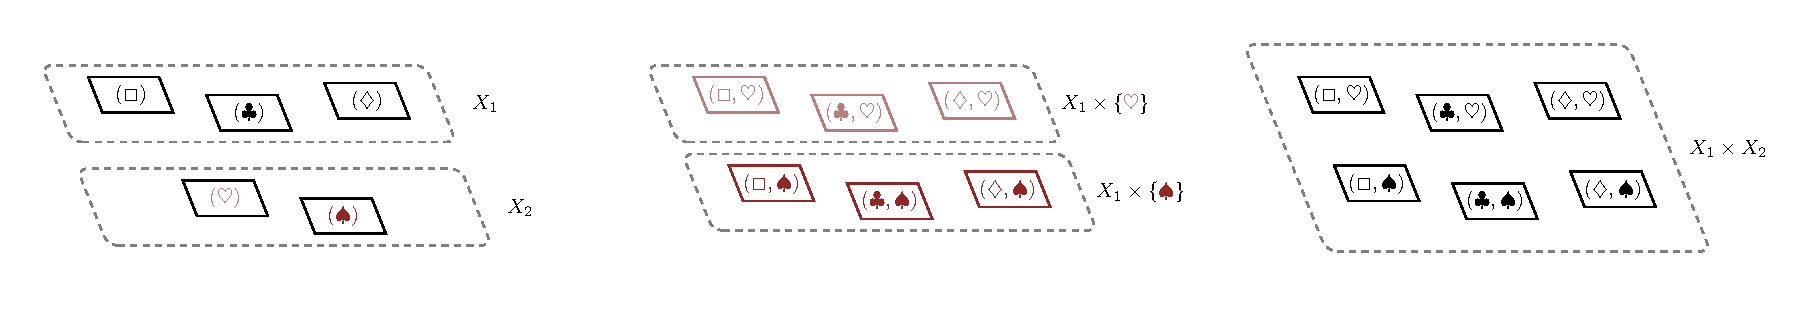
\includegraphics{figures/finite_product/X1_replications/X1_replications.pdf}

}

}

\subcaption{\label{fig-finite-product2}}
\end{minipage}%
%
\begin{minipage}[t]{0.05\linewidth}

{\centering 

~

}

\end{minipage}%
\newline
\begin{minipage}[t]{0.05\linewidth}

{\centering 

~

}

\end{minipage}%
%
\begin{minipage}[t]{0.90\linewidth}

{\centering 

\raisebox{-\height}{

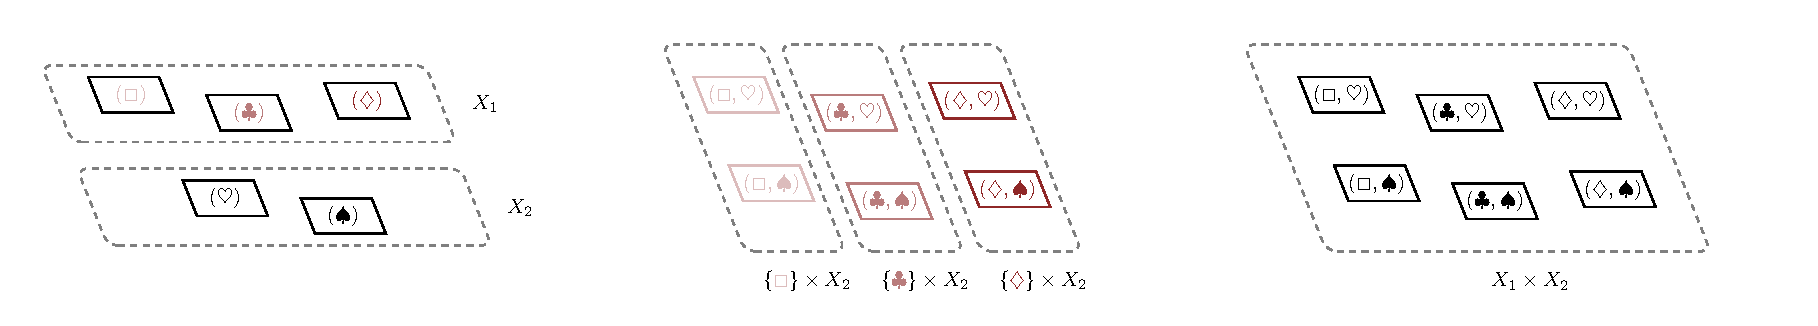
\includegraphics{figures/finite_product/X2_replications/X2_replications.pdf}

}

}

\subcaption{\label{fig-finite-product1}}
\end{minipage}%
%
\begin{minipage}[t]{0.05\linewidth}

{\centering 

~

}

\end{minipage}%

\caption{\label{fig-finite-product}The finite product set
\(X_{1} \times X_{2}\) can be constructed (a) by replicating the finite
set \(X_{2}\) once for each element of the finite set \(X_{1}\) or (b)
by replicating \(X_{1}\) once for each element of \(X_{2}\). Either way
results in an equivalent set of pairs of elements selected from
\(X_{1}\) and \(X_{2}\).}

\end{figure}

Each element of the product set is uniquely specified by one element of
\(X_{1}\) and one element of \(X_{2}\). Consequently every variable
taking values in the product set \(x \in X_{1} \times X_{2}\) is
compromised of an ordered pair of variables from each component space,
\[
x = (x_{1}, x_{2}),
\] with \(x_{1} \in X_{1}\) and \(x_{2} \times X_{2}\).

\hypertarget{general-product-sets}{%
\subsection{General Product Sets}\label{general-product-sets}}

This construction immediately generalizes beyond finite sets. Given two
sets \(X_{1}\) and \(X_{2}\) we can construct the product set by
replicating \(X_{2}\) once for each element of \(X_{1}\) and then
combining the replicated elements together
(Figure~\ref{fig-general-product2d-2}) \[
X_{1} \times X_{2} = \bigcup_{x_{1} \in X_{1}} \{ x_{1} \} \times X_{2},
\] or equivalently by replicating \(X_{1}\) once for each element of
\(X_{2}\) and then combining the replicated elements together
(Figure~\ref{fig-general-product2d-1}), \[
X_{1} \times X_{2} = \bigcup_{x_{2} \in X_{2}} X_{1} \times \{ x_{2} \}.
\] The common result \(X_{1} \times X_{2}\) is denoted a \textbf{product
set} with the \textbf{component sets} \(X_{1}\) and \(X_{2}\).

\begin{figure}

\begin{minipage}[t]{0.05\linewidth}

{\centering 

~

}

\end{minipage}%
%
\begin{minipage}[t]{0.90\linewidth}

{\centering 

\raisebox{-\height}{

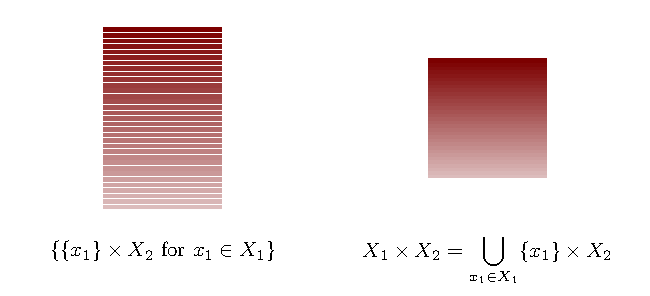
\includegraphics{figures/general_product/2d_X2_replications/2d_X2_replications.pdf}

}

}

\subcaption{\label{fig-general-product2d-2}}
\end{minipage}%
%
\begin{minipage}[t]{0.05\linewidth}

{\centering 

~

}

\end{minipage}%
\newline
\begin{minipage}[t]{0.05\linewidth}

{\centering 

~

}

\end{minipage}%
%
\begin{minipage}[t]{0.90\linewidth}

{\centering 

\raisebox{-\height}{

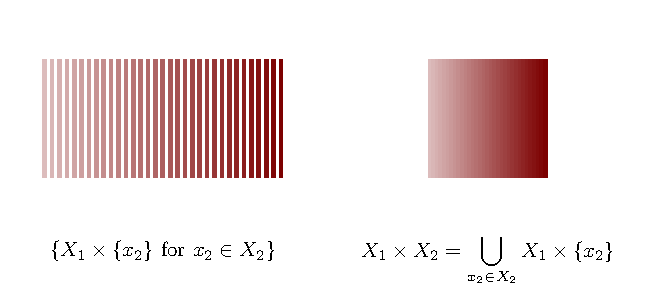
\includegraphics{figures/general_product/2d_X1_replications/2d_X1_replications.pdf}

}

}

\subcaption{\label{fig-general-product2d-1}}
\end{minipage}%
%
\begin{minipage}[t]{0.05\linewidth}

{\centering 

~

}

\end{minipage}%

\caption{\label{fig-general-product2d}A general product set with two
components \(X_{1} \times X_{2}\) can be constructed (a) by replicating
the set \(X_{2}\) once for each element of the set \(X_{1}\) or (b) by
replicating \(X_{1}\) once for each element of \(X_{2}\). Both
constructions give a set consisting of pairs of elements selected from
\(X_{1}\) and \(X_{2}\).}

\end{figure}

As in the finite case every element of a general, binary product set is
uniquely specified with a pair of elements, one from the first component
set, \(x_{1} \in X_{1}\), and the other from the second component set,
\(x_{2} \in X_{2}\). Because of this each variable taking values in the
product set \(x \in X_{1} \times X_{2}\) is comprised of an ordered pair
of component variables, \[
x = ( x_{1}, x_{2} )
\] with \(x_{1} \in X_{1}\) and \(x_{2} \in X_{2}\).

Iterating this construction allows us to define product sets from more
than two components sets. For example given three sets \(X_{1}\),
\(X_{2}\), and \(X_{3}\) we can construct the three-component product
space \(X_{1} \times X_{2} \times X_{3}\) in three equivalent different
ways (Figure~\ref{fig-general-product3d}). We can construct the product
set \(X_{1} \times X_{2}\) and then replicate it once for each element
\(x_{3} \in X_{3}\) before combining those replications together, \[
X_{1} \times X_{2} \times X_{3}
=
\bigcup_{ x_{3} \times X_{3} } X_{1} \times X_{2} \times \{ x_{3} \}.
\] At the same time we can construct the product set
\(X_{2} \times X_{3}\), replicate it once for each element
\(x_{1} \in X_{1}\), and the aggregate the resulting elements, \[
X_{1} \times X_{2} \times X_{3}
=
\bigcup_{ x_{1} \times X_{1} } \{ x_{1} \} \times X_{2} \times X_{3}.
\] Finally we can construct the product set \(X_{1} \times X_{3}\),
replicate it once for each element \(x_{2} \in X_{2}\), and then
aggregate, \[
X_{1} \times X_{2} \times X_{3}
=
\bigcup_{ x_{2} \times X_{2} } X_{1} \times \{ x_{2} \} \times X_{3}.
\] All three constructions result in the same product space where each
element is uniquely specified by a triplet of component variables, \[
x = (x_{1}, x_{2}, x_{3}).
\]

\begin{figure}

{\centering 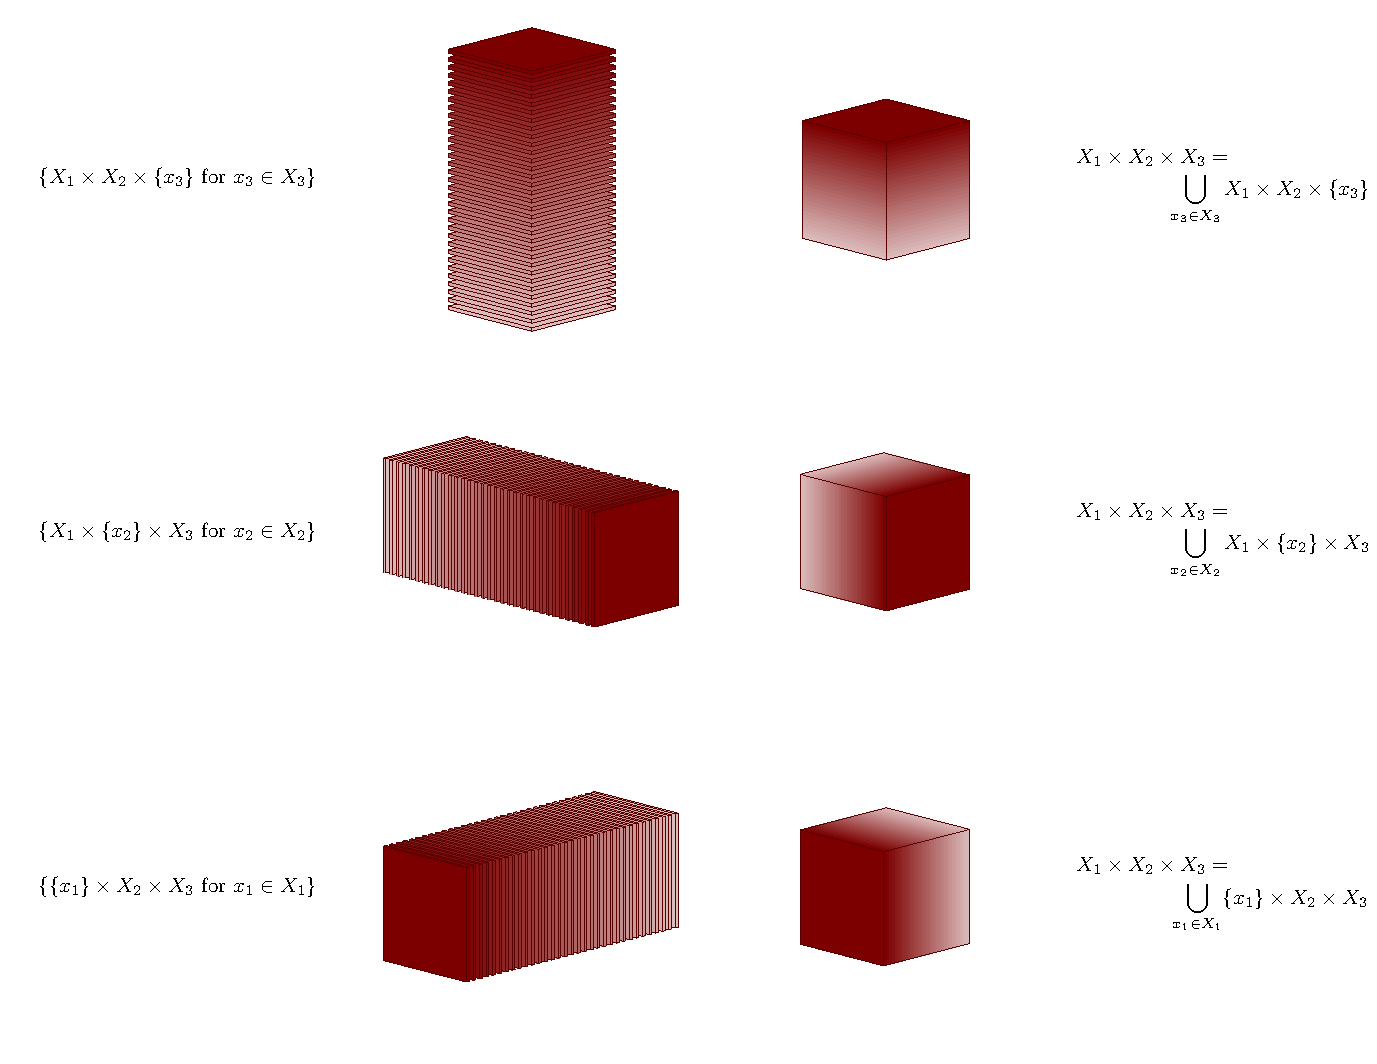
\includegraphics[width=0.9\textwidth,height=\textheight]{figures/general_product/3d_all/3d_all.pdf}

}

\caption{\label{fig-general-product3d}The three component sets
\(X_{1}\), \(X_{2}\), and \(X_{3}\) can be combined into the product set
\(X_{1} \times X_{2} \times X_{3}\) in multiple ways For example we can
first combine \(X_{1}\) and \(X_{2}\) into \(X_{1} \times X{2}\),
replicate that binary product once for each element of \(X_{3}\), and
then merge those replications. Alternatively we can combine \(X_{1}\)
and \(X_{3}\) first or \(X_{2}\) and then \(X_{3}\) first. All of these
constructions results in a three-component product space
\(X_{1} \times X_{2} \times X_{3}\).}

\end{figure}

More generally given \(I\) component sets \[
\{ X_{1}, \ldots, X_{i}, \ldots X_{I} \}
\] we can construct a corresponding product set \[
X_{1} \times \ldots \times X_{i} \times \ldots \times X_{I}
=
\times_{i = 1}^{I} X_{i}
\] where every product variable \(x \in \times_{i = 1}^{I} X_{i}\) is
compromised of a ordered collection of component variables \[
x = ( x_{1}, \ldots, x_{i}, \ldots, x_{I})
\] with \(x_{i} \in X_{i}\). This ordered collection of component
variables is known as an \textbf{n-tuple variable} or more compactly
just an \textbf{n-tuple}, generalizing ``couple'' that denotes a pair of
component variables and ``triple'' that denotes three component
variables to an arbitrary number of component variables. Because their
elements are specified by multiple variables product sets are often
referred to as \textbf{multivariate} sets.

When working with multiple product variables we might be inclined to use
integer indices to differentiate between them. These indices, however,
are readily confused with the indices used to denote the component
variables. In circumstances where numbering product variables is useful
I will use a comma to separate the indices with the first always
referring to the product variable and the latter always referring to the
component variable, \[
x_{j} = ( x_{j, 1}, \ldots, x_{j, i}, \ldots, x_{j, I}).
\] In other words \(x_{j, i}\) refers to the \(i\)th component variable
of the \(j\)th product variable.

\hypertarget{product-subsets}{%
\subsection{Product Subsets}\label{product-subsets}}

Just as elements from each of the component sets uniquely specifies an
element from the corresponding product set, a subset of the component
sets uniquely specifies a subset of the product set. These
\textbf{product subsets} \(\mathsf{x} \subset \times_{i = 1}^{I} X_{i}\)
are often written as \[
\mathsf{x}
=
\mathsf{x}_{1} \times \cdots \times
\mathsf{x}_{i} \times \cdots \times
\mathsf{x}_{I}
=
\times_{i = 1}^{I} \mathsf{x}_{i}
\] where \[
\mathsf{x}_{i} \subset X_{i}.
\]

The product power set is itself a product of the component power sets,
\[
2^{ \times_{i = 1}^{I} X_{i} }
=
2^{X_{1}} \times \ldots \times 2^{X_{i}} \times \ldots \times 2^{X_{I}}
=
\times_{i = 1}^{I} 2^{X_{i}}.
\] The empty product set is given by aggregating the component empty
sets, \[
\emptyset = \times_{i = 1}^{I} \emptyset_{i},
\] while the full product set is given by aggregating the component full
sets, \[
X = \times_{i = 1}^{I} X_{i}.
\]

Unfortunately most of the set operations are not compatible with the
component structure of a product set. For example the complement of a
product subset is not generally given by applying the complement
operation to each of the component subsets, \[
\mathsf{x}^{c} \ne \times_{i = 1}^{I} \mathsf{x}_{i}^{c},
\] although there are a few special cases where this is true. Similarly
the union of two product subsets is not generally given by the product
of the component unions: for two arbitrary product subsets \[
\mathsf{x} = \times_{i = 1}^{I} \mathsf{x}_{i}
\] and \[
\mathsf{x}' = \times_{i = 1}^{I} \mathsf{x}'_{i}
\] we will have \[
\mathsf{x} \cup \mathsf{x}'
\ne
\times_{i = 1}^{I} \mathsf{x}_{i} \cup \mathsf{x}'_{i}.
\] The lone exception is the intersection of product subsets, which can
always be derived from the intersection of the component subsets, \[
\mathsf{x} \cap \mathsf{x}'
=
\times_{i = 1}^{I} \mathsf{x}_{i} \cap \mathsf{x}'_{i}.
\]

This singular compatibility also introduces a convenient geometric
intuition to product subsets. In particular consider decomposing the
product subset \(X_{1} \times X_{2}\) into replications of \(X_{1}\), \[
X_{1} \times X_{2} = \bigcup_{x_{2} \in X_{2}} X_{1} \times \{ x_{2} \}.
\] Selecting the subset \(\mathsf{x}_{1} \subset X_{1}\) in every
replication \emph{lifts} \(\mathsf{x}_{1}\) into the product subset \[
\mathsf{x}_{1} \times X_{2} \subset X_{1} \times X_{2}.
\] At the same time given the decomposition \[
X_{1} \times X_{2} = \bigcup_{x_{1} \in X_{1}} \{ x_{1} \} \times X_{2}
\] we can select the subset \(\mathsf{x}_{2} \subset X_{2}\) in every
replication \(\{ x_{1} \} \times X_{2}\) to define the product subset \[
X_{1} \times \mathsf{x}_{2} \subset X_{1} \times X_{2}.
\] The intersection of these two lifted product subsets is then just the
product of \(\mathsf{x}_{1}\) and \(\mathsf{x}_{2}\), \begin{align*}
(\mathsf{x}_{1} \times X_{2}) \cap (X_{1} \times \mathsf{x}_{2})
&=
(\mathsf{x}_{1} \cap X_{1}) \times (X_{2} \cap \mathsf{x}_{2})
\\
&=
(\mathsf{x}_{1}) \times (\mathsf{x}_{2}).
\end{align*}

In other words we can interpret the product subset
\(\mathsf{x}_{1} \times \mathsf{x}_{2}\) as the overlap of the
``shadows'' that \(\mathsf{x}_{1}\) and \(\mathsf{x}_{2}\) cast into the
full product set (Figure~\ref{fig-product-set}). Because of this
geometric intuition product subsets are sometimes referred to as
\textbf{rectangular subsets}.

\begin{figure}

\begin{minipage}[t]{0.17\linewidth}

{\centering 

~

}

\end{minipage}%
%
\begin{minipage}[t]{0.66\linewidth}

{\centering 

\raisebox{-\height}{

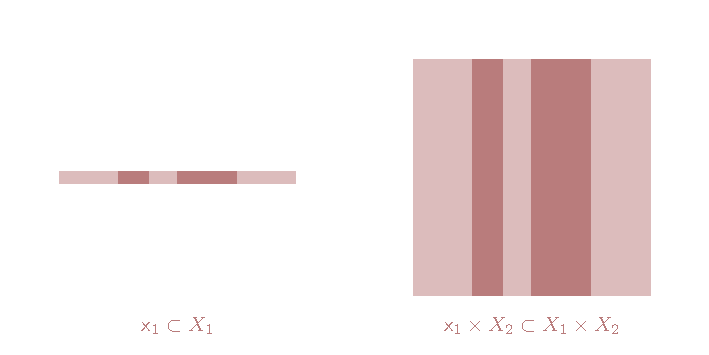
\includegraphics{figures/product_set/1/1.pdf}

}

}

\subcaption{\label{fig-product-set1}}
\end{minipage}%
%
\begin{minipage}[t]{0.17\linewidth}

{\centering 

~

}

\end{minipage}%
\newline
\begin{minipage}[t]{0.17\linewidth}

{\centering 

~

}

\end{minipage}%
%
\begin{minipage}[t]{0.66\linewidth}

{\centering 

\raisebox{-\height}{

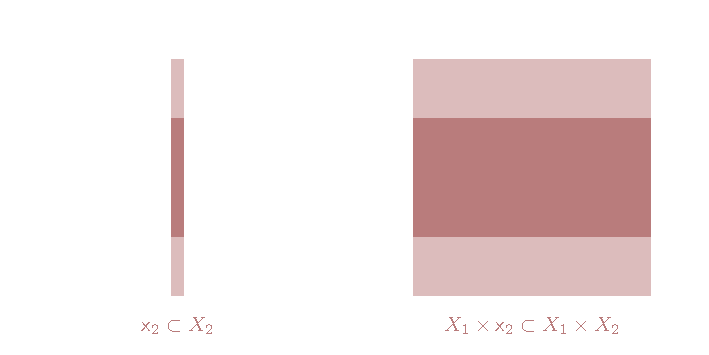
\includegraphics{figures/product_set/2/2.pdf}

}

}

\subcaption{\label{fig-product-set2}}
\end{minipage}%
%
\begin{minipage}[t]{0.17\linewidth}

{\centering 

~

}

\end{minipage}%
\newline
\begin{minipage}[t]{0.33\linewidth}

{\centering 

~

}

\end{minipage}%
%
\begin{minipage}[t]{0.34\linewidth}

{\centering 

\raisebox{-\height}{

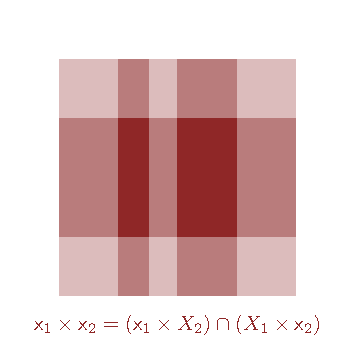
\includegraphics{figures/product_set/3/3.pdf}

}

}

\subcaption{\label{fig-product-set3}}
\end{minipage}%
%
\begin{minipage}[t]{0.33\linewidth}

{\centering 

~

}

\end{minipage}%

\caption{\label{fig-product-set}Product subsets admit a useful geometric
interpretation where (a, b) we first lift each component subset to the
product set before (c) constructing the product subset from their
overlap.}

\end{figure}

This geometric perspective can for example be used to better understand
why the complement and union operations aren't compatible with component
structure. The product of complementary component subsets generally
excludes all of the elements in the complement of the corresponding
product subset (Figure~\ref{fig-product-set-complement}). On the other
hand the product of the union of component subsets generally includes
elements that are not in the union of the corresponding product subsets
(Figure~\ref{fig-product-set-union}). Only when considering
intersections do both constructions always give the same subset
(Figure~\ref{fig-product-set-intersection}).

\begin{figure}

\begin{minipage}[t]{0.10\linewidth}

{\centering 

~

}

\end{minipage}%
%
\begin{minipage}[t]{0.80\linewidth}

{\centering 

\raisebox{-\height}{

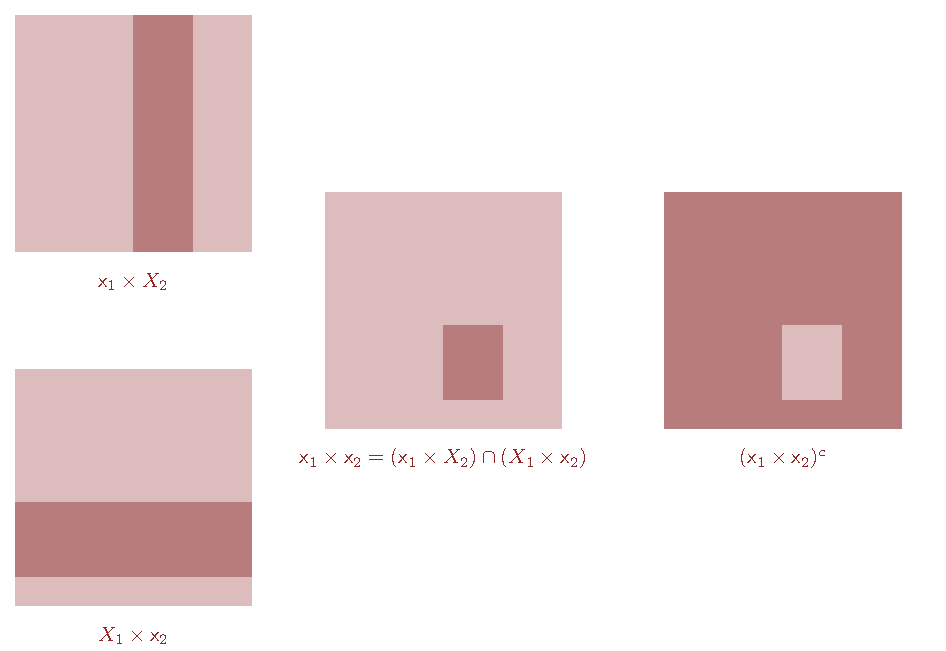
\includegraphics{figures/product_set_complement/pc/pc.pdf}

}

}

\subcaption{\label{fig-pc}}
\end{minipage}%
%
\begin{minipage}[t]{0.10\linewidth}

{\centering 

~

}

\end{minipage}%
\newline
\begin{minipage}[t]{0.10\linewidth}

{\centering 

~

}

\end{minipage}%
%
\begin{minipage}[t]{0.80\linewidth}

{\centering 

\raisebox{-\height}{

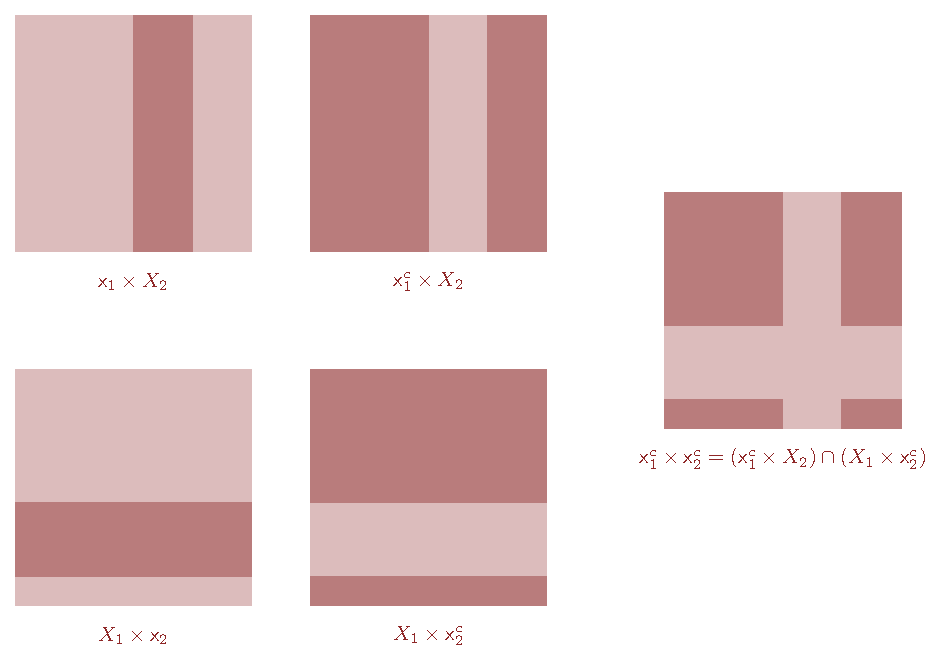
\includegraphics{figures/product_set_complement/cp/cp.pdf}

}

}

\subcaption{\label{fig-cp}}
\end{minipage}%
%
\begin{minipage}[t]{0.10\linewidth}

{\centering 

~

}

\end{minipage}%

\caption{\label{fig-product-set-complement}Combining component subsets
into a product subset doesn't commute with the complement operator. (a)
Taking the product first and then applying the complement operator
doesn't always give the same subset as (b) applying the complement
operator to each component subset and then taking their product.}

\end{figure}

\begin{figure}

\begin{minipage}[t]{0.15\linewidth}

{\centering 

~

}

\end{minipage}%
%
\begin{minipage}[t]{0.70\linewidth}

{\centering 

\raisebox{-\height}{

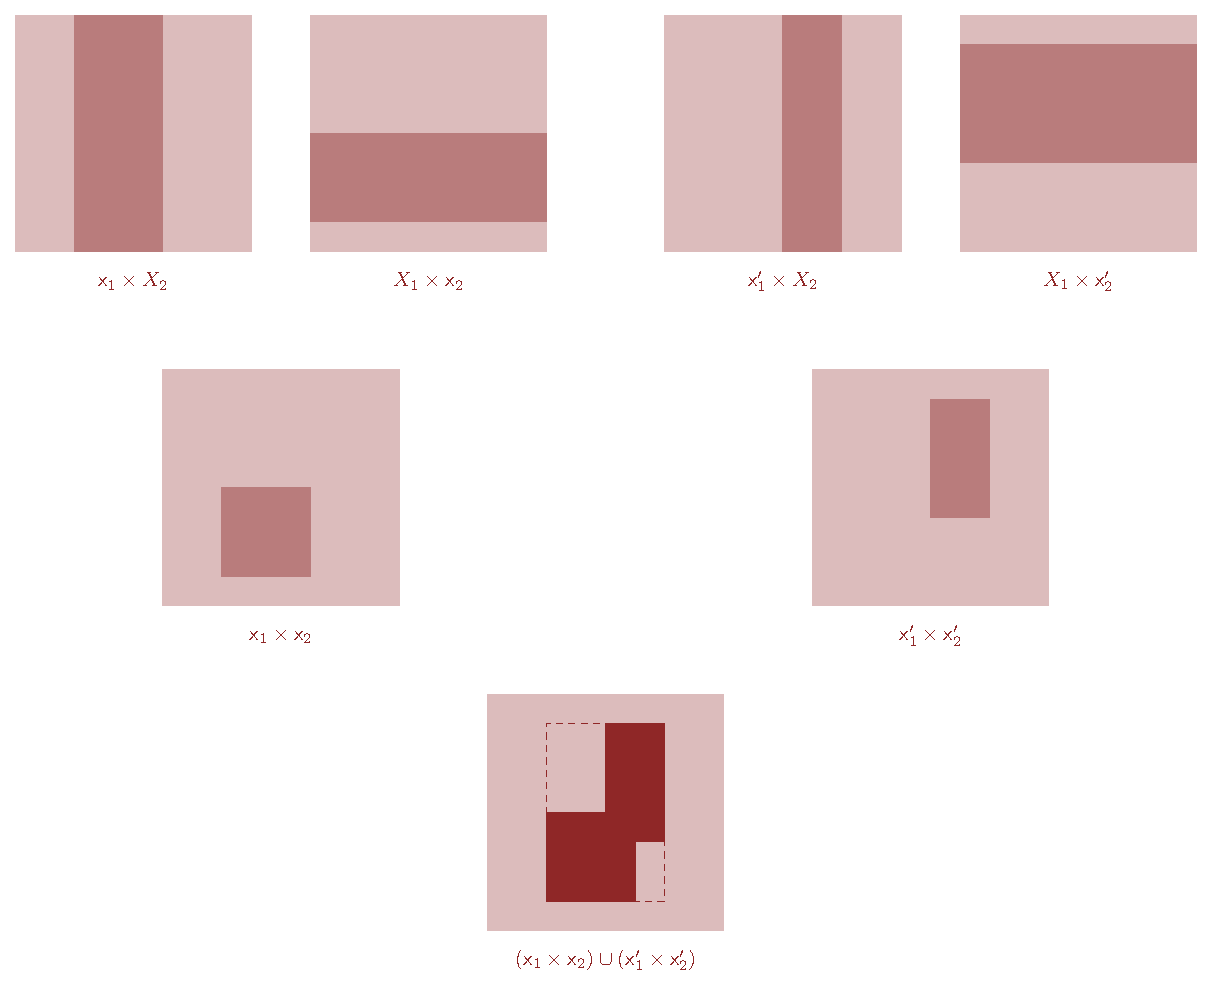
\includegraphics{figures/product_set_union/pu/pu.pdf}

}

}

\subcaption{\label{fig-pu}}
\end{minipage}%
%
\begin{minipage}[t]{0.15\linewidth}

{\centering 

~

}

\end{minipage}%
\newline
\begin{minipage}[t]{0.15\linewidth}

{\centering 

~

}

\end{minipage}%
%
\begin{minipage}[t]{0.70\linewidth}

{\centering 

\raisebox{-\height}{

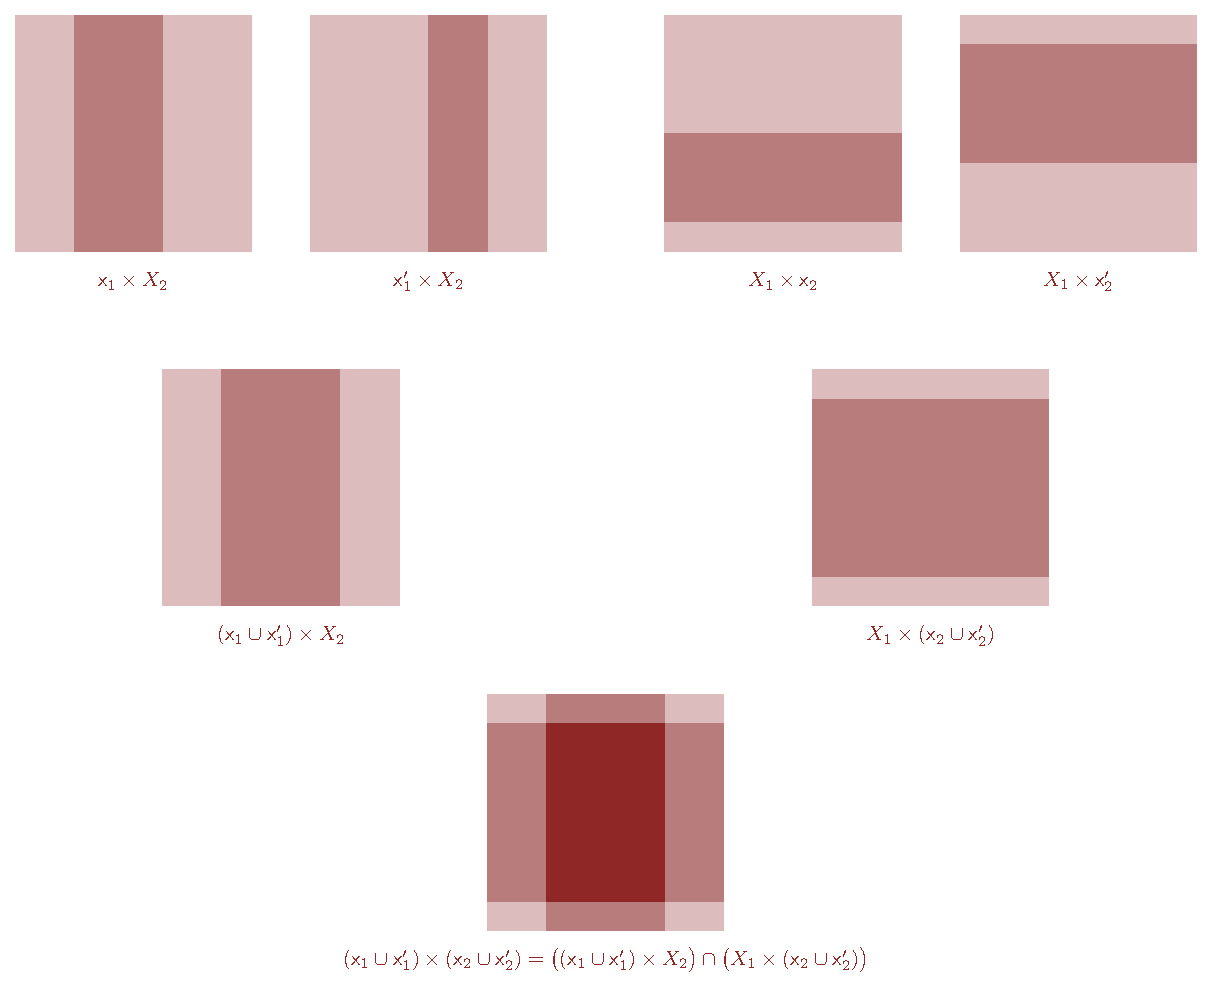
\includegraphics{figures/product_set_union/up/up.pdf}

}

}

\subcaption{\label{fig-up}}
\end{minipage}%
%
\begin{minipage}[t]{0.15\linewidth}

{\centering 

~

}

\end{minipage}%

\caption{\label{fig-product-set-union}The union operator also doesn't
commute with the product construction. (a) Taking the product first and
then applying the union operator doesn't always give the same subset as
(b) applying the union operator to each component subset and then taking
their product.}

\end{figure}

\begin{figure}

\begin{minipage}[t]{0.15\linewidth}

{\centering 

~

}

\end{minipage}%
%
\begin{minipage}[t]{0.70\linewidth}

{\centering 

\raisebox{-\height}{

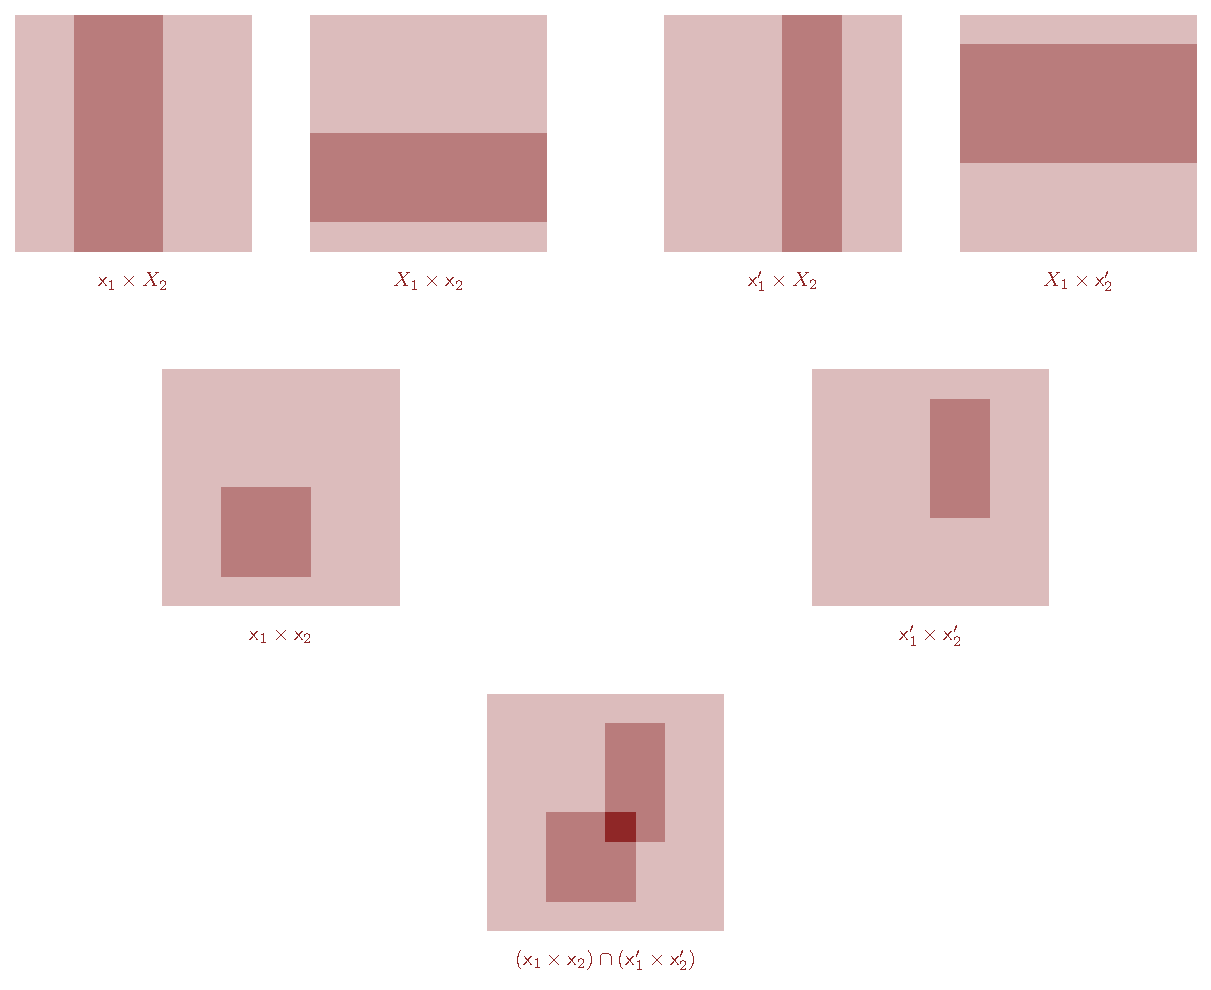
\includegraphics{figures/product_set_intersection/pi/pi.pdf}

}

}

\subcaption{\label{fig-pi}}
\end{minipage}%
%
\begin{minipage}[t]{0.15\linewidth}

{\centering 

~

}

\end{minipage}%
\newline
\begin{minipage}[t]{0.15\linewidth}

{\centering 

~

}

\end{minipage}%
%
\begin{minipage}[t]{0.70\linewidth}

{\centering 

\raisebox{-\height}{

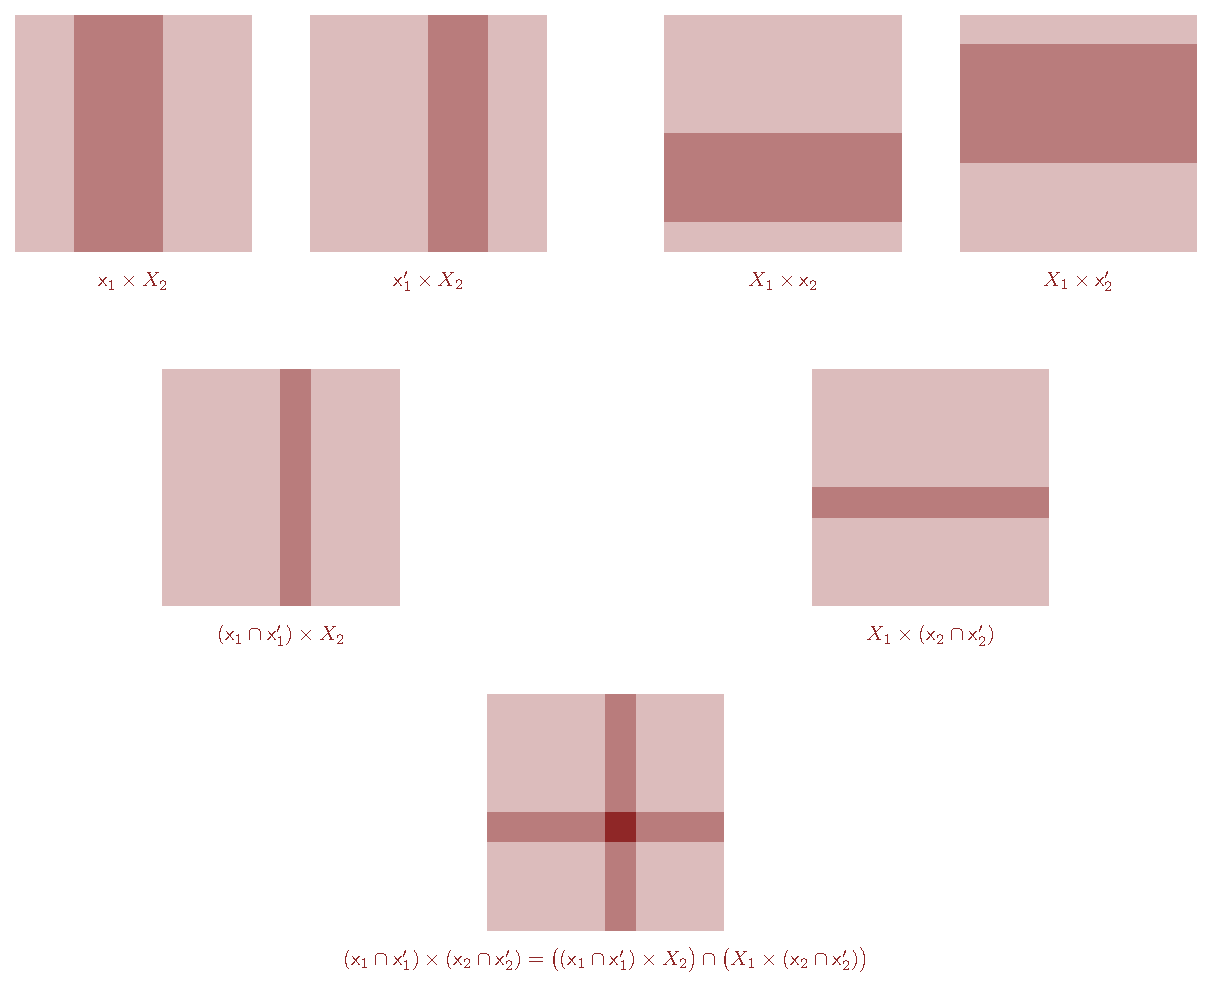
\includegraphics{figures/product_set_intersection/ip/ip.pdf}

}

}

\subcaption{\label{fig-ip}}
\end{minipage}%
%
\begin{minipage}[t]{0.15\linewidth}

{\centering 

~

}

\end{minipage}%

\caption{\label{fig-product-set-intersection}Of the three set operators
only the intersection operator commutes with products. (a) Taking the
product first and then applying the intersection operator always gives
the same subset as (b) applying the intersection operator to each
component subset and then taking their product.}

\end{figure}

Finally we need to keep in mind that, while they are very useful in
practice, product subsets do not span the entire product power set. In
other words not \emph{every} subset of \(\times_{i = 1}^{I} X_{i}\) is a
product subset. This includes for example the union of arbitrary product
subsets as well as many other, more intricate subsets of the product
set. Indeed most subsets of \emph{any} product set
\(\times_{i = 1}^{I} X_{i}\) are not product subsets!

\hypertarget{product-structure}{%
\section{Product Structure}\label{product-structure}}

In order to elevate product \emph{sets} to product \emph{spaces} we need
to construct product \emph{structure} from any structure endowed onto
the component sets. Conveniently these constructions are straightforward
for our basic structures.

In this section I will always assume the ambient product set
\(X = \times_{i = 1}^{I} X_{i}\) with component sets \(X_{i}\).

\hypertarget{product-orderings}{%
\subsection{Product Orderings}\label{product-orderings}}

If each component set is equipped with a strict ordering then we can
unambiguously define a product variable \(x \in X\) to be smaller than
another product variable \(x' \in X\) if \emph{all} of the component
elements in \(x\) are smaller than \emph{all} of the corresponding
component elements in \(x'\). In other words \(x < x'\) if and only if
\[
x_{i} < x'_{i}
\] for all \(i \in {1, \ldots, I}\).

On the other hand if only \emph{some} of the component elements in \(x\)
are smaller than the corresponding component elements in \(x'\), while
some are larger, then the comparison between the two product elements
will be ambiguous. Consequently a strict ordering on the component sets
does not fully define a strict ordering on the product set.

That said we can use the strict component orderings to define a partial
ordering of the product set where any two product elements with mixed
component orderings are arranged together. In the same way we can use
partial component orderings to define a partial ordering of the product
set. Either way component orderings will generally define partial
product orderings.

\hypertarget{product-algebras}{%
\subsection{Product Algebras}\label{product-algebras}}

When each component set is equipped with an individual algebraic
operation we can define a corresponding product operation by applying
these component operations at the same time. For example if each
component set is equipped with a binary operation \begin{alignat*}{6}
\cdot_{i} :\; & X_{i} \times X_{i}& &\rightarrow& \; & X_{i} &
\\
& x_{i}, x'_{i} & &\mapsto& & x_{i} \cdot x'_{i} &,
\end{alignat*} then we can construct a \textbf{product operation}
\(\cdot : X \times X \rightarrow X\) as \[
x \cdot x' =
( x_{1} \cdot_{1} x'_{1}, \ldots,
  x_{i} \cdot_{i} x'_{i}, \ldots,
  x_{I} \cdot_{I} x'_{I} ).
\]

Product operations acquire any properties that are shared by \emph{all}
of the component operations. For example if all of the component
operations are commutative then the product operation will also be
commutative. Similarly if all of the component operations are unital
with identity elements \(x_{\text{Id}, i}\) then the product operation
will also be unital with the composite identity element \[
x_{\text{Id}} = (x_{\text{Id}, 1}, \ldots,
                 x_{\text{Id}, i}, \ldots,
                 x_{\text{Id}, I}).
\]

\hypertarget{product-metrics}{%
\subsection{Product Metrics}\label{product-metrics}}

Product metrics can be constructed by summing over the outputs of
component metrics. More formally if each component set is equipped with
a metric \begin{alignat*}{6}
d_{i} :\; & X_{i} \times X_{i}& &\rightarrow& \; & \mathbb{R}^{+} &
\\
& x_{i}, x'_{i} & &\mapsto& & d(x_{i}, x'_{i}) &
\end{alignat*} then we can define a \textbf{product metric} as
\begin{alignat*}{6}
d :\; & X \times X& &\rightarrow& \; & \mathbb{R}^{+} &
\\
& x, x' & &\mapsto& & \sum_{i = 1}^{I} d(x_{i}, x'_{i}). &
\end{alignat*}

Critically this product metric acquires all of the properties required
of a metric from the component metrics. By construction the product
distances vanish if and only if all of the individual component
distances vanish. This requires all of the component elements to be
equal which implies that the product elements are also equal. In other
words the product metric returns zero if and only if the two input
product elements are the same, as required for a metric.

On the other hand two input product elements are distinct if and only if
at least one of the component element has to be distinct. In this case
at least one of the component distances will be greater than zero.
Consequently the summed distances will be non-zero whenever the input
product elements are distinct.

Symmetry of the product metric follows the commutativity of the
component metrics, \begin{align*}
d(x, x')
&= \sum_{i = 1}^{I} d(x_{i}, x'_{i})
\\
&= \sum_{i = 1}^{I} d(x'_{i}, x_{i})
\\
&= d(x', x).
\end{align*} Likewise for any three product elements
\(x, x', x'' \in X\) we always have a triangle inequality,
\begin{align*}
d(x, x'')
&=
\sum_{i = 1}^{I} d(x_{i}, x''_{i})
\\
&\le
\sum_{i = 1}^{I} d(x_{i}, x'_{i}) + d(x'_{i}, x''_{i})
\\
&\le
\sum_{i = 1}^{I} d(x_{i}, x'_{i}) + \sum_{i = 1}^{I} d(x'_{i}, x''_{i})
\\
&\le
d(x, x') + d(x', x'').
\end{align*}

\hypertarget{product-topologies}{%
\subsection{Product Topologies}\label{product-topologies}}

If every component set is equipped with a component topology
\(\mathfrak{t}_{i}\) then we can define open component subsets
\(\mathsf{x}_{i} \in \mathfrak{t}_{i}\). Any combination of these open
component subsets then defines an \textbf{open product subset} \[
\times_{i = 1}^{I} \mathsf{x}_{i}.
\]

Because the component topologies all contain the component empty sets
and component full sets we will always be able to construct the product
empty set and product full set from this procedure.

Moreover because the component open subsets are finite intersections
these productsubsets will be as well. For example given any finite
collection of open component subsets \[
\{ \mathsf{x}_{1, i}, \ldots, \mathsf{x}_{j, i}, \ldots \mathsf{x}_{J, i} \}
\] we have closure under intersections, \[
\mathsf{x}_{\cup, i}
\equiv \cap_{j = 1}^{J} \mathsf{x}_{j, i}
\in \mathfrak{t}_{i}.
\] Consequently the intersection of any finite collection of open
product subsets gives another open product subset, \begin{align*}
\cap_{j} \mathsf{x}_{j}
&=
\cap_{j} \left( \times_{i = 1}^{I} \mathsf{x}_{j, i} \right)
\\
&=
\times_{i = 1}^{I} \left( \cap_{j} \mathsf{x}_{j, i} \right)
\\
&=
\times_{i = 1}^{I} \left( \mathsf{x}_{\cup, i} \right).
\end{align*}

Unfortunately the union of any open product subsets will not in general
be another product subset. Combining the open product subsets with all
of their unions, however, defines a collection of subsets that satisfies
all of the properties of a topology. We refer to this topology as a
\textbf{product topology}.

\hypertarget{prototypical-product-spaces}{%
\section{Prototypical Product
Spaces}\label{prototypical-product-spaces}}

The most common product spaces we will encounter in practice are built
up from the prototypical spaces that we reviewed in
\href{@sec:proto-spaces}{Chapter 2, Section 2}, combining various
integers and real lines together into larger spaces. That said there are
a few product spaces worth particular note.

\hypertarget{replicated-product-spaces}{%
\subsection{Replicated Product Spaces}\label{replicated-product-spaces}}

Often we are interested not in any single element of a space \(X\) but
rather multiple elements of that space at the same time. The selection
of \(I\) elements can be modeled by replicating the space \(I\) times
and then using those replications as components of a product space, \[
X^{I} = X \times \ldots \times X = \times_{i = 1}^{I} X.
\] This construction is referred to as a \textbf{replicated product
space}, \textbf{identical product space} or \textbf{power space}.

We already have seen this construction in a few places. For example we
defined binary algebraic operator over the set \(X\) as mapping two
elements of \(X\) into a single element of \(X\). That input set of
pairs of elements was denoted \(X \times X\), which is just a replicated
product set with a separate copy of \(X\) for each input.

Similarly sequences of \(I\) elements from a given set, \[
\{ x_{1}, \ldots, x_{i}, \ldots, x_{I} \},
\] can be defined as elements of the replicated power set \(X^{I}\).
Allowing \(I\) to become arbitrarily large then allows for the countably
infinitely long s equences.

One potential difficulty that can arise when working with replicated
product spaces is distinguishing between the different copies of the
base space \(X\) that form the components. In particular any notation
that might differentiate the individual copies, such as ticks or integer
indices, can also be confused as defining different spaces entirely. For
example depending on the context \(X_{1} \times X_{2}\) might be used to
denote both a product space comprised of two \emph{different} spaces and
a replicated product space comprised of two copies of the \emph{same}
space. To avoid any confusion we have to be explicit about when we are
assuming a general product space and when we are assuming a replicated
product space.

\hypertarget{multivariate-real-numbers}{%
\subsection{Multivariate Real Numbers}\label{multivariate-real-numbers}}

Combining \(I\) real lines together defines the \textbf{multivariate
real numbers}, \(\mathbb{R}^{I}\). This is also referred to as a
\textbf{real space} or an \textbf{\(I\)-dimensional Euclidean space}.

The multivariate real numbers inherit the identity crisis of the real
lines from which they are built. If we take the perspective that there
are infinite, distinct real lines then there will be infinite, distinct
multivariate real numbers: different choices of component ordering,
algebraic, and metric structures will define distinct product spaces. On
the other hand if we assume that there is a single, flexible real line
that admits multiple configurations then the multivariate real numbers
will correspond to a single, flexible space. In this case each different
configuration of the component lines will define a different
configuration of the corresponding product space.

To visually summarize the structure of a real space we can extend grids
defined over the component spaces across the other component spaces and
then overlay them to form a rectangular \emph{mesh}
(Figure~\ref{fig-real_space_grid}).

\begin{figure}

{\centering 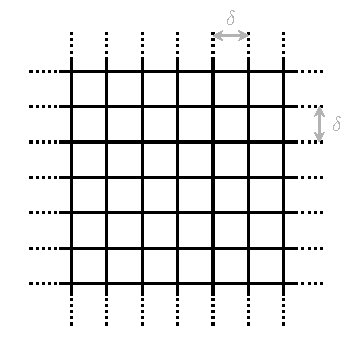
\includegraphics[width=0.5\textwidth,height=\textheight]{figures/real_space_grid/real_space_grid.pdf}

}

\caption{\label{fig-real_space_grid}Extending component grids into the
product space defines a rectangular mesh that visually communicate the
product metric structure. Here \(\mathbb{R}^{2}\) is represented by a
two-dimensional mesh.}

\end{figure}

\hypertarget{sec:decomposition}{%
\section{Decomposing Product Spaces}\label{sec:decomposition}}

Every element of a product space is uniquely specified by an element
from each component space. Specifying all of the component elements at
the same time, however, can sometimes be overwhelming. Fortunately we
can always specify the component elements \emph{sequentially}.

For example if we decompose a two component product set
\(X_{1} \times X_{2}\) into replications of the second component set, \[
X_{1} \times X_{2} = \bigcup_{x_{1} \in X_{1} } \{ x_{1} \} \times X_{2}
\] then every element can be specified by first specifying an element of
the first component set, \[
\tilde{x}_{1} \in X_{1},
\] and then an element in the corresponding replication of the second
component set, \[
x_{2} \in \{ \tilde{x}_{1} \} \times X_{2},
\] to give \[
(\tilde{x}_{1}, \tilde{x}_{2}) \in X_{1} \times X_{2}.
\] Note that we're using the \(\tilde{}\) here to denote bound variables
as we make each choice of component elements.

At the same time if we decompose the product set into \[
X_{1} \times X_{2} = \bigcup_{x_{2} \in X_{2} } X_{1} \times \{ x_{2} \}
\] then every element can be specified by first specifying an element of
the second component set, \[
\tilde{x}_{2} \in X_{2},
\] before specifying an element in the corresponding replication of the
first component set, \[
\tilde{x}_{1} \in X_{1} \times \{ x_{2} \}.
\]

This sequential specification also has a nice geometric interpretation
(Figure~\ref{fig-sequential-selection}). Specifying
\(\tilde{x}_{1} \in X_{1}\) and then
\(\tilde{x}_{2} \in \{ \tilde{x}_{1} \} \times X_{2}\) corresponds to
arriving at \((\tilde{x}_{1}, \tilde{x}_{2})\) by first moving along
\(X_{1}\) and then moving along the replication
\(\{ x_{1} \} \times X_{2}\). Alternatively specifying
\(\tilde{x}_{2} \in X_{2}\) and then
\(\tilde{x}_{1} \in X_{1} \times \{ \tilde{x}_{2} \}\) corresponds to
moving along \(X_{2}\) before moving along \(\{ x_{1} \} \times X_{2}\).

\begin{figure}

\begin{minipage}[t]{0.05\linewidth}

{\centering 

~

}

\end{minipage}%
%
\begin{minipage}[t]{0.90\linewidth}

{\centering 

\raisebox{-\height}{

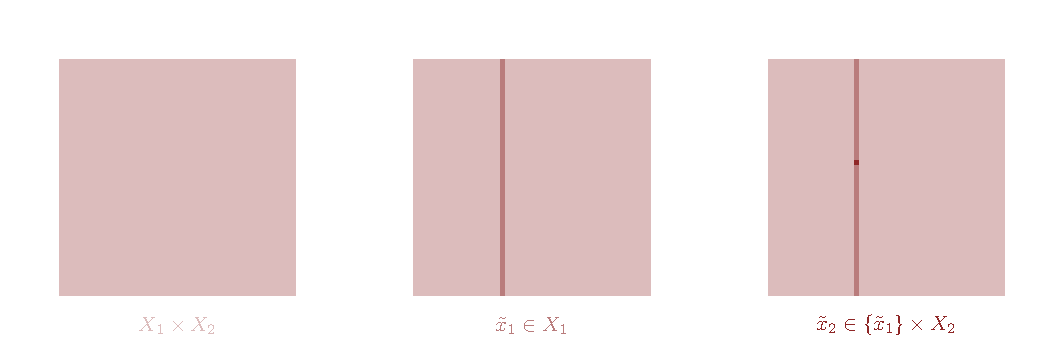
\includegraphics{figures/sequential_selection/12/12.pdf}

}

}

\subcaption{\label{fig-sequential-selection12}}
\end{minipage}%
%
\begin{minipage}[t]{0.05\linewidth}

{\centering 

~

}

\end{minipage}%
\newline
\begin{minipage}[t]{0.05\linewidth}

{\centering 

~

}

\end{minipage}%
%
\begin{minipage}[t]{0.90\linewidth}

{\centering 

\raisebox{-\height}{

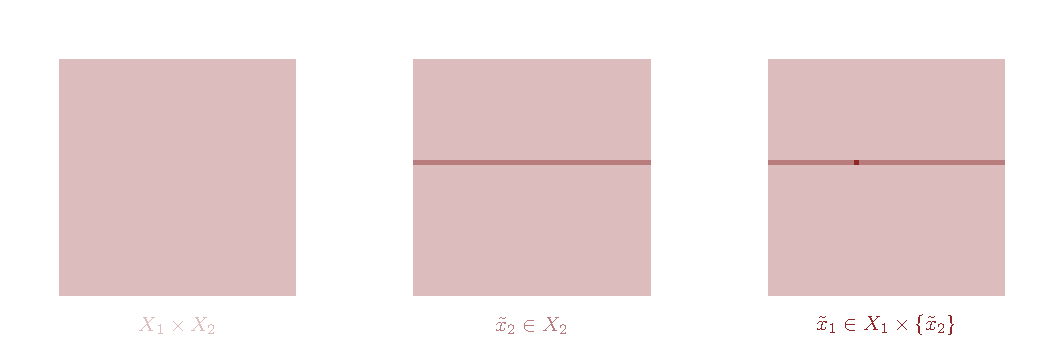
\includegraphics{figures/sequential_selection/21/21.pdf}

}

}

\subcaption{\label{fig-sequential-selection21}}
\end{minipage}%
%
\begin{minipage}[t]{0.05\linewidth}

{\centering 

~

}

\end{minipage}%

\caption{\label{fig-sequential-selection}The element
\((\tilde{x}_{1}, \tilde{x}_{2}) \in X_{1} \times X_{2}\) can be
constructed sequentially in two different ways. (a) We can restrict our
initial attention to \(X_{1}\) to select \(\tilde{x}_{1} \in X_{1}\) and
then consider the corresponding replication to select
\(\{ x_{1} \} \times X_{2}\). (b) Alternatively we could first select
\(\tilde{x}_{2} \in X_{2}\) before selecting
\(\tilde{x}_{1} \in X_{1} \times \{ \tilde{x}_{2} \}\).}

\end{figure}

We have even more options for sequentially selecting component elements
from a product set with three components. For example if we decompose
the product set into replications of \(X_{1} \times X_{2}\) \[
X_{1} \times X_{2} \times X_{3}
=
\bigcup_{ x_{3} \times X_{3} } X_{1} \times X_{2} \times \{ x_{3} \}.
\] then we can specify an element by first taking an element of the
third component set, \[
\tilde{x}_{3} \in X_{3},
\] and then an element of the corresponding replication, \[
(\tilde{x}_{1}, \tilde{x}_{2}) \in X_{1} \times X_{2} \times \{ x_{3} \},
\] to give \[
(\tilde{x}_{1}, \tilde{x}_{2}, \tilde{x}_{3}) \in X_{1} \times X_{2} \times X_{3}.
\] By decomposing \(X_{1} \times X_{2}\), however, the latter
specification can further be separated into \[
\tilde{x}_{2} \in X_{2} \times \{ \tilde{x}_{3} \}
\] and then \[
\tilde{x}_{1} \in X_{1} \times \{ \tilde{x}_{2} \} \times \{ \tilde{x}_{3} \},
\] or \[
\tilde{x}_{1} \in X_{1} \times \{ \tilde{x}_{3} \}
\] and then \[
\tilde{x}_{2} \in \{ \tilde{x}_{1} \} \times X_{2} \times \{ \tilde{x}_{3} \}.
\] The different ways that we can initially decompose
\(X_{1} \times X_{2} \times X_{3}\) allow us to specify an element of
the product set by specifying component elements \emph{in any order}.

This pattern immediately generalizes to any product space. Unfortunately
the generalization quickly become complicated because of all of the ways
that we can select from the available components. To represent how we
can sequentially build up product elements from component elements we'll
need some careful, if a bit ungainly, notation.

We'll start with the \(I\) component spaces \[
X_{1}, \ldots, X_{i}, \ldots, X_{I},
\] which together form the total product space \begin{align*}
\times_{i = 1}^{I} X_{i}
&= \times_{i \in (1, \ldots, I )} X_{i}
\\
&= X_{1} \times \ldots \times X_{i} \times \ldots \times X_{I}.
\end{align*} I will refer to this as the \textbf{joint set}.

At the same time any selection of those \(I\) components also defines a
smaller product set: for any collection of \(J < I\) component indices
\[
( i_{1}, \ldots, i_{J} )
\] we can construct the product set \[
\times_{ i' \in ( i_{1}, \ldots, i_{J} ) } X_{i'}
=
X_{i_{1}} \times \ldots \times X_{i_{J}}.
\] I will refer to these as \textbf{marginal sets}.

If we select the components \(( i_{1}, \ldots, i_{J} )\) then the
remaining components, \[
( 1, \ldots, i_{1} - 1, i_{1} + 1, \ldots, i_{J} - 1, i_{J} + 1, \ldots, J )
\] define yet another product set. Replicating this second product set
once for each element of first product defines a collection of
\textbf{conditional sets} (Figure~\ref{fig-conditioning}),
\begin{align*}
\times_{i' = 1}^{I} X_{i'} \mid (x_{i_{1}}, \ldots, x_{i_{J}})
&\equiv \quad
X_{1} \times \ldots
\\
&\quad \times
X_{i_{1} - 1} \times \{ x_{i_{1}} \} \times X_{i_{1} + 1} \times \ldots
\\
&\quad \times
X_{i_{J} - 1} \times \{ x_{i_{J}} \} \times X_{i_{J} + 1} \times \ldots
\\
&\quad \times X_{I}.
\end{align*} In other words the elements of a conditional set are given
by taking an element of the joint set and then fixing, or
\emph{conditioning}, the component elements of the corresponding
marginal set.

\begin{figure}

{\centering 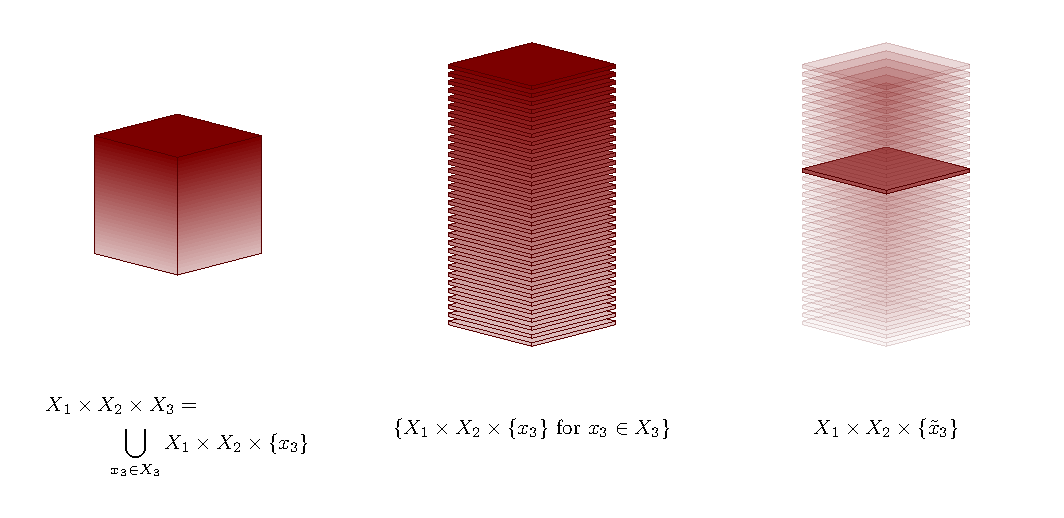
\includegraphics[width=0.9\textwidth,height=\textheight]{figures/conditioning/conditioning.pdf}

}

\caption{\label{fig-conditioning}A product set can be decomposed into
various combinations of marginal sets and conditional sets. For example
taking \(X_{3}\) as a marginal set reduces the three-component product
set \(X_{1} \times X_{2} \times X_{3}\) into the conditional sets
\(X_{1} \times X_{2} \times \{ x_{3} \}\), one for each element of the
marginal set. Fixing a particular element \(\tilde{x}_{3} \in X_{3}\)
isolates one of those replications.}

\end{figure}

A marginal set and its complementary collection of conditional sets can
then be used to reconstruct the joint set, \[
\times_{i = 1}^{I} X_{i}
=
\bigcup_{ (x_{i_{1}}, \ldots, x_{i_{J}}) \in \times_{ i' \in ( i_{1}, \ldots, i_{J} ) } X_{i'} }
\left( \times_{i' = 1}^{I} X_{i'} \right) \mid (x_{i_{1}}, \ldots, x_{i_{J}}).
\] This then allows us to specify an element of the joint set \[
(\tilde{x}_{1}, \ldots, \tilde{x}_{i_{1}}, \ldots, \tilde{x}_{i_{J}}, \ldots, \tilde{x}_{I})
\in \times_{i = 1}^{I} X_{i}.
\] by first specifying a collection of component elements, \[
(\tilde{x}_{i_{1}}, \ldots, \tilde{x}_{i_{J}})
\in \times_{ i' \in ( i_{1}, \ldots, i_{J} ) } X_{i'},
\] and then specifying the remaining component elements in the
corresponding replication, \begin{align*}
&(\tilde{x}_{1}, \ldots,
\tilde{x}_{i_{1} - 1}, \tilde{x}_{i_{1} + 1}, \ldots,
\tilde{x}_{i_{J} - 1}, \tilde{x}_{i_{J} + 1}, \ldots,
\tilde{x}_{I} )
\\
&\hspace{35mm} \in
\left( \times_{i' = 1}^{I} X_{i'} \right) \mid (\tilde{x}_{i_{1}}, \ldots, \tilde{x}_{i_{J}}).
\end{align*} Because we have to account for any choice of marginal set
the notation here is far from elegant, but keep in mind that all we're
doing is formalizing what happens when we select some component elements
first and then the remaining elements second.

Given any partition of the component sets into groups we can apply this
decomposition \emph{recursively} to decompose the joint set into a
sequence of collections of conditional sets and one terminating marginal
set. For example consider five component sets
\(X_{1}, X_{2}, X_{3}, X_{4}, X_{5}\) which are partitioned into three
groups, \[
\{ X_{2}, X_{5} \}, \{ X_{3} \}, \{X_{1}, X_{4} \}.
\] This partition motivates the decomposition \begin{align*}
&X_{1} \times X_{2} \times X_{3} \times X_{4} \times X_{5}
\\
&\hspace{10mm} =
\bigcup_{ (x_{2}, x_{5}) \in X_{2} \times X_{5} }
\bigcup_{ x_{3} \in X_{3} \mid (x_{2}, x_{5}) }
X_{1} \times X_{4} \mid (x_{2}, x_{3}, x_{5})
\end{align*} and the corresponding sequential specification
\begin{align*}
(\tilde{x}_{2}, \tilde{x}_{5}) &\in
X_{2} \times X_{5}
\\
\tilde{x}_{3} &\in
X_{3} \mid (\tilde{x}_{2}, \tilde{x}_{5})
\\
(\tilde{x}_{1}, x_{4}) &\in
X_{1} \times X_{4} \mid (\tilde{x}_{2}, \tilde{x}_{3}, \tilde{x}_{5}).
\end{align*}

In most applications we will want to separate the component sets
individually, allowing us to build a joint element up by specifying
component elements one by one. For example working through the component
spaces in order gives the specification \begin{alignat*}{3}
\tilde{x}_{1} &\in  X_{1} &&
\\
\tilde{x}_{2} &\in X_{2} &\mid& \; \tilde{x}_{1}
\\
&\ldots
\\
\tilde{x}_{i} &\in X_{i} &\mid& \; ( \tilde{x}_{1}, \ldots, \tilde{x}_{i} )
\\
&\ldots
\\
\tilde{x}_{I - 1} &\in X_{I - 1} &\mid& \; ( \tilde{x}_{1}, \ldots, \tilde{x}_{I - 2} )
\\
\tilde{x}_{I} &\in X_{I} &\mid& \; ( \tilde{x}_{1}, \ldots, \tilde{x}_{I - 1} ).
\end{alignat*} That said we can work through the component spaces in
\emph{any} order. This flexibility allows us to construct joint elements
in whichever way is most convenient in a given application.

Because we often take sequential specification of elements for granted
this formal, systematic treatment might appear to be a
bit\ldots excessive. To the contrary this more careful perspective will
help us understand some of the more subtle aspects of probability theory
on product spaces, and how we can develop sophisticated probability
distributions in practice.

\hypertarget{transforming-product-spaces}{%
\section{Transforming Product
Spaces}\label{transforming-product-spaces}}

We can always transform product spaces directly with monolithic maps
that ignore any component structure. These functions map an entire input
product set to an arbitrary output set, \begin{alignat*}{6}
f :\; & \times_{i = 1}^{I} X_{i} & &\rightarrow& \; & Y &
\\
& (x_{1}, \ldots, x_{i}, \ldots, x_{I}) & &\mapsto&
& y = f(x_{1}, \ldots, x_{i}, \ldots, x_{I}) &.
\end{alignat*}

For example algebraic operations can be interpreted as functions from
the input replicated product set \(X \times X\) to the output set \(X\),
\begin{alignat*}{6}
f :\; & X \times X & &\rightarrow& \; & X &
\\
& (x_{1}, x_{2}) & &\mapsto& & x = f(x_{1}, x_{2}) &.
\end{alignat*} Similarly metrics can be interpreted as functions from
that same input product set to an output positive real line,
\begin{alignat*}{6}
d :\; & X \times X & &\rightarrow& \; & \mathbb{R}^{+} &
\\
& (x_{1}, x_{2}) & &\mapsto& & d(x_{1}, x_{2}) &.
\end{alignat*}

The classification of these functions and construction of pushforward
and pullback functions follows exactly the same as for functions with
general input spaces. We can say much more, however, about functions
that naturally harmonize with the component structure of an input
product space.

\hypertarget{component-transformations}{%
\subsection{Component Transformations}\label{component-transformations}}

Transformations between two product spaces exhibit a useful
fragmentation. Any function between two product sets \begin{alignat*}{6}
f :\; & \times_{i = 1}^{I} X_{i} & &\rightarrow& \; & \times_{j = 1}^{J} Y_{j} &
\\
& (x_{1}, \ldots, x_{i}, \ldots, x_{I}) & &\mapsto&
& (y_{1}, \ldots, y_{j}, \ldots, y_{J}) = f(x_{1}, \ldots, x_{i}, \ldots, x_{I}) &
\end{alignat*} is equivalent to \(J\) functions that map the input
product set into each of the individual output component sets,
\begin{alignat*}{6}
f_{j} :\; & \times_{i = 1}^{I} X_{i} & &\rightarrow& \; & Y_{j} &
\\
& (x_{1}, \ldots, x_{i}, \ldots, x_{I}) & &\mapsto&
& y_{j} = f_{j}(x_{1}, \ldots, x_{i}, \ldots, x_{I}) &.
\end{alignat*} Pushforward and pullback maps for the complete function
can be derived from these component functions.

In general these component functions mix the input components together
to inform the behavior in each output component set. Some functions,
however, limit each of the input component sets to informing only a
single output component set. Specifically if the input product set and
output product set are built up from the same number of component sets
\(I\) then some functions will map only one input component into each of
the output components at a time, \begin{alignat*}{6}
f_{i} :\; & X_{i} & &\rightarrow& \; & Y_{i} &
\\
& x_{i} & &\mapsto& & y_{i} = f_{i}(x_{i}) &.
\end{alignat*} These component-preserving functions transform each
component \emph{independently} of the others.

One nice feature of component-preserving transformations is that they
preserve the orientation of grids defined from any component metric
structure. For example the function \begin{alignat*}{6}
f :\; & \mathbb{R}^{2} & &\rightarrow& \; & \mathbb{R}^{2} &
\\
& (x_{1}, x_{2}) & &\mapsto& &
(y_{1}, y_{2}) = (x_{1}^{\frac{3}{2}}, x_{2}^{\frac{3}{2}}) &
\end{alignat*} transforms \(x_{1}\) into \(y_{1}\) independently of the
behavior of \(x_{2}\) and similarly transforms \(x_{2}\) into \(y_{2}\)
independently of the behavior of \(x_{1}\). While neither of these
component transformations are isometries the rectangular structure of
any metric-informed grid will be preserved
(Figure~\ref{fig-pushforward-grids1}).

On the other hand the function \begin{alignat*}{6}
f :\; & \mathbb{R}^{2} & &\rightarrow& \; & \mathbb{R}^{2} &
\\
& (x_{1}, x_{2}) & &\mapsto& & (y_{1}, y_{2} = (x_{1} + x_{2}, x_{1} - x_{2}) &
\end{alignat*} mixes the input components \(x_{1}\) and \(x_{2}\)
together, skewing the product structure in the process. Consequently
grids built up from the component metric structures on the input and
output spaces will appear \emph{warped} relative to each other
(Figure~\ref{fig-pushforward-grids2}).

\begin{figure}

\begin{minipage}[t]{0.05\linewidth}

{\centering 

~

}

\end{minipage}%
%
\begin{minipage}[t]{0.90\linewidth}

{\centering 

\raisebox{-\height}{

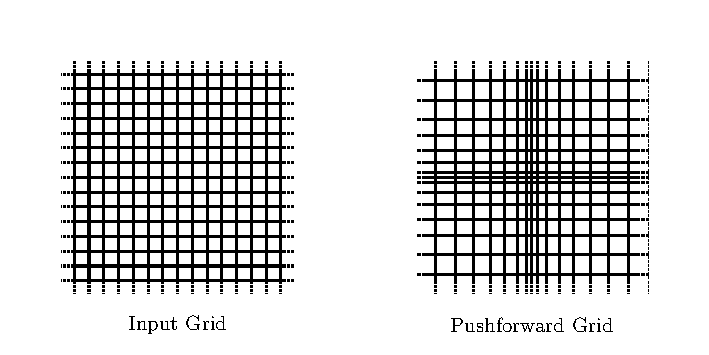
\includegraphics{figures/pushforward_grids/rectangular/rectangular.pdf}

}

}

\subcaption{\label{fig-pushforward-grids1}}
\end{minipage}%
%
\begin{minipage}[t]{0.05\linewidth}

{\centering 

~

}

\end{minipage}%
\newline
\begin{minipage}[t]{0.05\linewidth}

{\centering 

~

}

\end{minipage}%
%
\begin{minipage}[t]{0.90\linewidth}

{\centering 

\raisebox{-\height}{

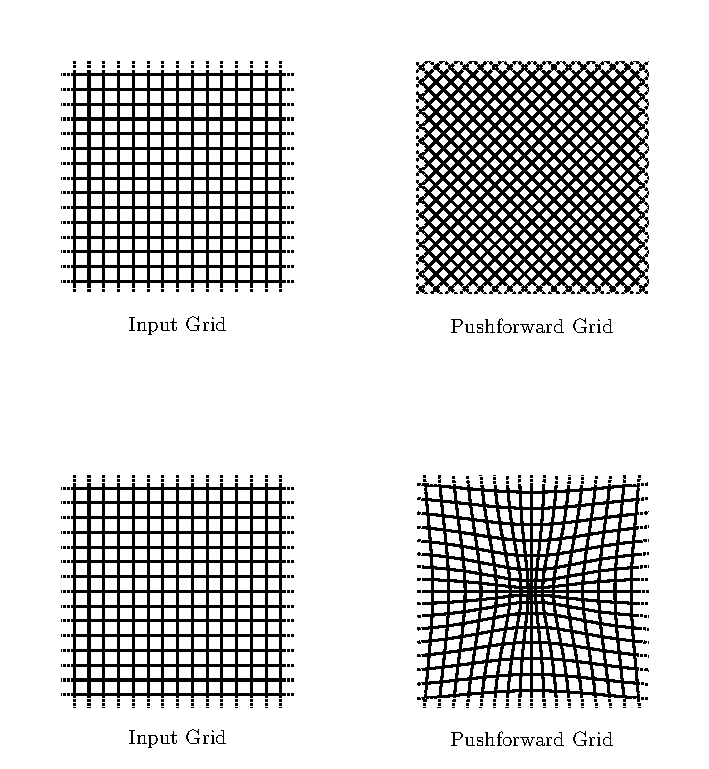
\includegraphics{figures/pushforward_grids/warped/warped.pdf}

}

}

\subcaption{\label{fig-pushforward-grids2}}
\end{minipage}%
%
\begin{minipage}[t]{0.05\linewidth}

{\centering 

~

}

\end{minipage}%

\caption{\label{fig-pushforward-grids}Maps between product metric spaces
may or may not preserve the individual components, and this has
consequences for how metric-informed grids transform. (a) Maps between
product metric spaces that do preserve the components transform
rectangular grids into rectangular grids. (b) On the other hand maps
that mix the components transform rectangular grids into grids that
appear rotated, skewed, or otherwise warped.}

\end{figure}

The behavior of component-preserving functions is completely determined
by the behavior of the component functions. For example a
component-preserving function is injective, surjective, or bijective if
and only if all of the component functions are injective, surjective, or
bijective. Similarly any product structure endowed on the input product
set will be preserved if each of the component structures are preserved
along the component transformations.

\hypertarget{projection-functions}{%
\subsection{Projection Functions}\label{projection-functions}}

The component-structure of a product space naturally motivates an
important class of functions. Consider, for example, the two-component
product space \(X_{1} \times X_{2}\) and its decomposition into distinct
replications of \(X_{1}\), \[
X_{1} \times X_{2} = \bigcup_{x_{2} \in X_{2}} X_{1} \times \{ x_{2} \}.
\] If we ignore the \(x_{2}\) label the replications
\(X_{1} \times \{ x_{2} \}\) become indistinguishable from each other,
collapsing into a single copy of \(X_{1}\)
(Figure~\ref{fig-projection}). This collapse \emph{projects} every
element of the product set \((x_{1}, x_{2}) \in X_{1} \times X_{2}\) to
a component element \(x_{1} \in X_{1}\).

At the same time we can decompose the product set into replications of
\(X_{2}\), \[
X_{1} \times X_{2} = \bigcup_{x_{1} \in X_{1}} \{ x_{1} \} \times X_{2}.
\] Ignoring the \(x_{1}\) label collapses the replications
\(\{ x_{1} \} \times X_{2}\) onto each other, projecting every product
element \((x_{1}, x_{2}) \in X_{1} \times X_{2}\) to the component
\(x_{2} \in X_{2}\).

\begin{figure}

{\centering 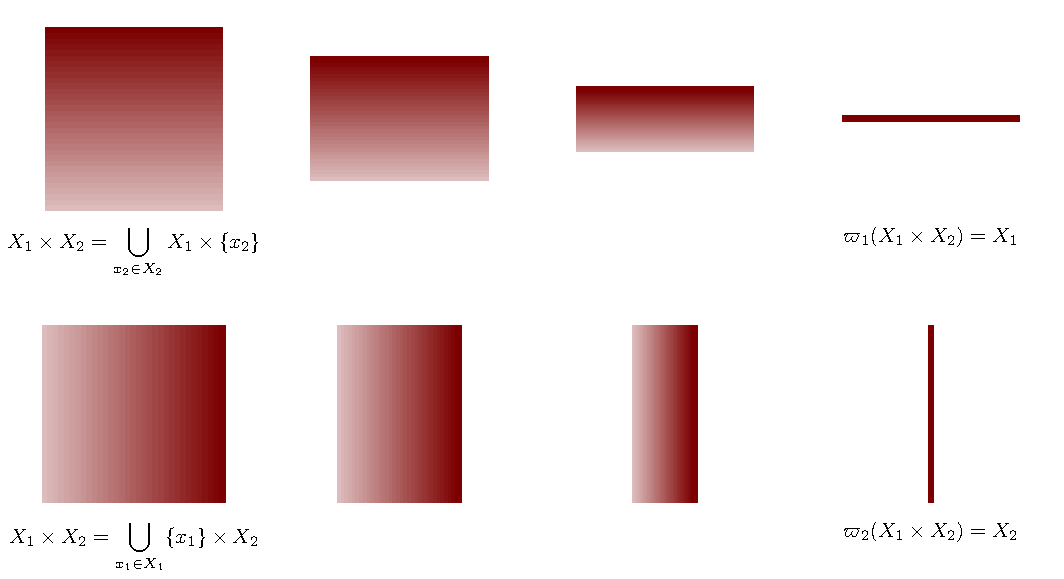
\includegraphics[width=0.9\textwidth,height=\textheight]{figures/projection/projection.pdf}

}

\caption{\label{fig-projection}Decomposing a product set into
replications and then collapsing those replications on top of each other
returns one of the component sets. This allows us to project a product
set onto any of its components.}

\end{figure}

More generally every product set is accompanied by surjective
\textbf{projection functions} that map the entire product set into the
individual component sets by ignoring the other components,
\begin{alignat*}{6}
\varpi_{i} :\; & \times_{i' = 1}^{I} X_{i'} & &\rightarrow& \; & X_{i} &
\\
& (x_{1}, \ldots, x_{i}, \ldots, x_{I}) & &\mapsto& & x_{i} &.
\end{alignat*}

These projections functions are fully consistent with any structure
endowed onto the product set. For example the pushforward of any product
structure along a projection functions returns the component structure
that was used to construct that product structure in the first place.
Similarly the pullback of any component structure along a projection
function will be always be compatible with the corresponding product
structure.

We can also construct more sophisticated \textbf{multi-projection
functions} that return multiple component spaces at the same time. In
particular given \(J < I\) component indices
\(( i_{1}, \ldots, i_{J} )\) we can define a projection function that
maps the product of all of the component sets into a product of just
those selected component sets, \begin{alignat*}{6}
\varpi_{i_{1}, \ldots, i_{J}} :\; & \times_{i' = 1}^{I} X_{i'} & &\rightarrow& \;
& \times_{ i' \in ( i_{1}, \ldots, i_{J} ) } X_{i'} &
\\
& (x_{1}, \ldots, x_{I}) & &\mapsto& & (x_{i}, x_{j}, x_{k}) &.
\end{alignat*}

Projection functions are particularly useful for succinctly expressing
some of the more subtle product space behaviors. As we saw in the
previous section every function with a product space input decomposes
into component functions, \begin{alignat*}{6}
f_{j} :\; & \times_{i = 1}^{I} X_{i} & &\rightarrow& \; & Y_{j} &
\\
& (x_{1}, \ldots, x_{i}, \ldots, x_{I}) & &\mapsto&
& y_{j} = f_{j}(x_{1}, \ldots, x_{i}, \ldots, x_{I}) &.
\end{alignat*} Those component functions, however, can be directly
defined as the composition of \(f\) with each projection function on the
output space, \[
f_{j} = \varpi_{j} \circ f.
\]

Similarly the marginal sets that we introduced in
\href{@sec:decomposition}{Section 4} can also be defined as the outputs
of various multi-projection functions. Even better every conditional set
can be defined as the preimage of a particular multi-projection
function, \[
\times_{i' = 1}^{I} X_{i'} \mid (x_{i_{1}}, \ldots, x_{i_{J}})
=
\varpi_{i_{1}, \ldots, i_{J}}^{-1}(x_{i_{1}}, \ldots, x_{i_{J}})!
\] In other words a conditional set can be defined as the subset of the
joint set that projects to a particular element of a marginal set. This
projection perspective not only clarifies why marginal and conditional
sets are complementary but also provides a compact way of denoting these
sets.

\hypertarget{partial-evaluation}{%
\subsection{Partial Evaluation}\label{partial-evaluation}}

Fully evaluating a function on a product space requires the
specification of an element in \emph{every} component space. For example
in order to evaluate the function \[
f: X_{1} \times X_{2} \rightarrow Y
\] we need to specify \(\tilde{x}_{1} \in X_{1}\) and
\(\tilde{x}_{2} \in X_{2}\) to define the particular output element \[
f(\tilde{x}_{1}, \tilde{x}_{2}) = y \in Y.
\]

Providing only one element leaves an empty slot in the input product set
that we need to fill in order to complete the evaluation. For example
\(f(\tilde{x}_{1}, x_{2})\) still needs an element of \(X_{2}\) and
\(f(x_{1}, \tilde{x}_{2})\) still needs an element of \(X_{1}\). That
empty slot, however, defines a relationship between the missing input
component set and the output set. In other words
\(f(\tilde{x}_{1}, x_{2})\) implicitly defines a function that maps
elements of\(\{ \tilde{x}_{1} \} \times X_{2}\) to elements of \(Y\).
Similarly \(f(x_{1}, \tilde{x}_{2})\) implicitly defines a function that
maps elements of \(X_{1} \times \{ \tilde{x}_{2} \}\) to elements of
\(Y\).

More generally specifying the component elements \[
( \tilde{x}_{i_{1}}, \ldots, \tilde{x}_{i_{J}} )
\] reduces to the product set \(\times_{i' = 1}^{I} X_{i'}\) to the
conditional set \[
\times_{i' = 1}^{I} X_{i'} \mid (\tilde{x}_{i_{1}}, \ldots, \tilde{x}_{i_{J}}).
\] Likewise inputting those component elements into a function
\begin{alignat*}{6}
f :\; & \times_{i = 1}^{I} X_{i} & &\rightarrow& \; & Y &
\\
& (x_{1}, \ldots, x_{i}, \ldots, x_{I}) & &\mapsto&
& y = f(x_{1}, \ldots, x_{i}, \ldots, x_{I}) &
\end{alignat*} defines a new function that maps the remaining elements
to an output element, \begin{alignat*}{6}
f_{ \tilde{x}_{i_{1}}, \ldots, \tilde{x}_{i_{J}} } :\; &
\times_{i' = 1}^{I} X_{i'} \mid (\tilde{x}_{i_{1}}, \ldots, \tilde{x}_{i_{J}}) &
&\rightarrow& \; & Y &
\\
& (x_{1}, \ldots, x_{i_{1} - 1}, x_{i_{1} + 1}, \ldots, & &\mapsto&
& y = f(x_{1}, \ldots, x_{i_{1} - 1}, \tilde{x}_{i_{1}}, x_{i_{1} + 1}, \ldots, &
\\
& \;\, x_{i_{J} - 1}, x_{i_{J} + 1}, \ldots, x_{I} \quad\quad) & &\mapsto&
& \quad\quad\quad x_{i_{J} - 1}, \tilde{x}_{i_{J}}, x_{i_{J} + 1}, \ldots, x_{I} \quad\quad) &.
\end{alignat*}

This procedure is known as \textbf{partial evaluation} generally and
\textbf{Currying} in the computer science literature particularly. The
mathematical notation for a partially evaluated function can vary quite
a bit. Besides \[
f_{\tilde{x}_{i_{1}}, \ldots, \tilde{x}_{i_{J}}}
\] it is not uncommon to see notation like \[
f(\cdot \mid \tilde{x}_{i_{1}}, \ldots, \tilde{x}_{i_{J}})
\] where \(\cdot\) represents the remaining unbound variables or even
notation that explicity writes out all of the bound and unbound
variables, \[
f(x_{1}, \ldots, x_{i_{1} - 1}, \tilde{x}_{i_{1}}, x_{i_{1} + 1}, \ldots,
x_{i_{J} - 1}, \tilde{x}_{i_{J}}, x_{i_{J} + 1}, \ldots,
x_{I} ).
\] While this latter notation is most direct it quickly becomes ungainly
when working with more than a few components.

Like the sequential specification of product set elements the partial
evaluation of functions is often taken for granted in practical
applications. Explicitly acknowledging it, however, can help us better
understand less obvious constructions.

For example consider a set \(X\) equipped with a binary addition
operator \begin{alignat*}{6}
+ :\; & X \times X& &\rightarrow& \; & X &
\\
& x_{1}, x_{2} & &\mapsto& & x_{1} + x_{2} &.
\end{alignat*} Partially evaluating this function on the first input
component effectively defines a function \begin{alignat*}{6}
t_{\tilde{x}_{1}} :\; &X& &\rightarrow& \; & X &
\\
& x_{2} & &\mapsto& & \tilde{x}_{1} + x_{2} &
\end{alignat*} that \emph{translates} each element of \(X\) by
\(\tilde{x}_{1}\). Consequently \(t_{\tilde{x}_{1}}\) is referred to as
a translation operator.

Similarly if we have a set \(X\) equipped with a binary multiplication
operator \begin{alignat*}{6}
\cdot :\; & X \times X& &\rightarrow& \; & X &
\\
& x_{1}, x_{2} & &\mapsto& & x_{1} \cdot x_{2} &
\end{alignat*} then partial evaluation effectively defines a function
\begin{alignat*}{6}
s_{\tilde{x}_{1}} :\; &X& &\rightarrow& \; & X &
\\
& x_{2} & &\mapsto& & \tilde{x}_{1} \cdot x_{2} &
\end{alignat*} that \emph{scales} each element of \(X\) by
\(\tilde{x}_{1}\). Fittingly \(s_{\tilde{x}_{1}}\) is often referred to
as a scaling operator.

We implicitly reason about translations and scalings in many
applications, but partial evaluation allows us to formalize that
conceptual reasoning. This more formal construction then helps us
recognize the necessary assumptions for that reasoning to be
well-defined. For example translation isn't well-defined on a space that
isn't equipped with the right algebraic structure!

\hypertarget{conclusion}{%
\section{Conclusion}\label{conclusion}}

The construction of product spaces defines a systematic way to work with
multiple elements from multiple spaces at the same time, or even
multiple elements from a single space at the same time. This has many
practical benefits. For example it facilitates the development and
manipulation of the sophisticated spaces we often need for applied
mathematical modeling. At the same time it provides a language for
formalizing certain computational techniques.

When working with more than a few component spaces some of the details
of the formal construction of product spaces -- such as the sequential
specification of product elements, projections, and partial evaluations
-- require some less-than-elegant notation. That said this awkwardness
is not due to any conceptual complexity so much as the difficulty in
enumerating all of the ways that we can select from a general collection
of component spaces.

\hypertarget{acknowledgements}{%
\section*{Acknowledgements}\label{acknowledgements}}
\addcontentsline{toc}{section}{Acknowledgements}

I thank Alexander Noll for helpful comments.

A very special thanks to everyone supporting me on Patreon: Adam
Fleischhacker, Adriano Yoshino, Alan Chang, Alessandro Varacca,
Alexander Bartik, Alexander Noll, Alexander Petrov, Alexander Rosteck,
Anders Valind, Andrea Serafino, Andrew Mascioli, Andrew Rouillard,
Andrew Vigotsky, Angie\_Hyunji Moon, Ara Winter, Austin Rochford, Austin
Rochford, Avraham Adler, Ben Matthews, Ben Swallow, Benjamin Glemain,
Bradley Kolb, Brynjolfur Gauti Jónsson, Cameron Smith, Canaan Breiss,
Cat Shark, Charles Naylor, Chase Dwelle, Chris Zawora, Christopher
Mehrvarzi, Chuck Carlson, Colin Carroll, Colin McAuliffe, Cruz, Damien
Mannion, Damon Bayer, dan mackinlay, Dan Muck, Dan W Joyce, Dan Waxman,
Dan Weitzenfeld, Daniel Edward Marthaler, Daniel Rowe, Darshan Pandit,
Darthmaluus , David Burdelski, David Galley, David Humeau, David Wurtz,
dilsher singh dhillon, Doug Rivers, Dr.~Jobo, Dr.~Omri Har Shemesh, Ed
Cashin, Ed Henry, Edgar Merkle, edith darin, Eric LaMotte, Erik Banek,
Ero Carrera, Eugene O'Friel, Felipe González, Fergus Chadwick, Finn
Lindgren, Florian Wellmann, Francesco Corona, Geoff Rollins, Greg
Sutcliffe, Guido Biele, Hamed Bastan-Hagh, Haonan Zhu, Hector Munoz,
Henri Wallen, hs, Hugo Botha, Håkan Johansson, Ian Costley, Ian Koller,
idontgetoutmuch, Ignacio Vera, Ilaria Prosdocimi, Isaac Vock, J, J
Michael Burgess, Jair Andrade, James Hodgson, James McInerney, James
Wade, Janek Berger, Jason Martin, Jason Pekos, Jason Wong, Jeff Burnett,
Jeff Dotson, Jeff Helzner, Jeffrey Erlich, Jesse Wolfhagen, Jessica
Graves, Joe Wagner, John Flournoy, Jonathan H. Morgan, Jonathon Vallejo,
Joran Jongerling, Joseph Despres, Josh Weinstock, Joshua Duncan, Joshua
Griffith, Josué Mendoza, JU, Justin Bois, Karim Naguib, Karim Osman,
Kejia Shi, Kevin Foley, Kristian Gårdhus Wichmann, Kádár András, lizzie
, LOU ODETTE, Marc Dotson, Marcel Lüthi, Marek Kwiatkowski, Mark
Donoghoe, Mark Worrall, Markus P., Martin Modrák, Matt Moores, Matthew,
Matthew Kay, Matthieu LEROY, Maurits van der Meer, Merlin Noel
Heidemanns, Michael DeWitt, Michael Dillon, Michael Lerner, Mick Cooney,
Márton Vaitkus, N Sanders, Name, Nathaniel Burbank, Nic Fishman,
Nicholas Clark, Nicholas Cowie, Nick S, Nicolas Frisby, Octavio Medina,
Ole Rogeberg, Oliver Crook, Olivier Ma, Pablo León Villagrá, Patrick
Kelley, Patrick Boehnke, Pau Pereira Batlle, Peter Smits, Pieter van den
Berg , ptr, Putra Manggala, Ramiro Barrantes Reynolds, Ravin Kumar, Raúl
Peralta Lozada, Riccardo Fusaroli, Richard Nerland, RLW, Robert Frost,
Robert Goldman, Robert kohn, Robert Mitchell V, Robin Taylor, Ross
McCullough, Ryan Grossman, Rémi , S Hong, Scott Block, Scott Brown, Sean
Pinkney, Sean Wilson, Seth Axen, shira, Simon Duane, Simon Lilburn,
Srivatsa Srinath, sssz, Stan\_user, Stefan, Stephanie Fitzgerald,
Stephen Lienhard, Steve Bertolani, Stone Chen, Susan Holmes, Svilup,
Sören Berg, Tao Ye, Tate Tunstall, Tatsuo Okubo, Teresa Ortiz, Thomas
Lees, Thomas Vladeck, Tiago Cabaço, Tim Radtke, Tobychev , Tom McEwen,
Tony Wuersch, Utku Turk, Virginia Fisher, Vitaly Druker, Vladimir
Markov, Wil Yegelwel, Will Farr, Will Tudor-Evans, woejozney, Xianda
Sun, yolhaj , yureq , Zach A, Zad Rafi, and Zhengchen Cai.

\hypertarget{license}{%
\section*{License}\label{license}}
\addcontentsline{toc}{section}{License}

A repository containing all of the files used to generate this chapter
is available on
\href{https://github.com/betanalpha/quarto_chapters/tree/main/8_product_spaces}{GitHub}.

The text and figures in this chapter are copyrighted by Michael
Betancourt and licensed under the CC BY-NC 4.0 license:

https://creativecommons.org/licenses/by-nc/4.0/



\end{document}
